Selon le fait \ref{nece-cond}, si parmi les \ngones\ de périmètre fixé, il en existe un qui maximise l'aire, alors ce ne peut être que le \ngone\ régulier. Nous allons établir que cette condition nécessaire est suffisante. Pour cela, nous avons juste besoin de savoir qu'il existe au moins un \ngone\ d'aire maximale.
Comme dans la remarque \ref{tri-topo-comp}, nous allons convier le couple continuité/compacité, mais ici les choses se compliquent, car nous allons devoir accepter de travailler avec des polygones croisés, et par conséquent il nous faut un moyen de mesurer la surface de tels polygones (le vrai point délicat est ici). 
Plaçons-nous d'un point de vue informatique: comme on sait calculer l'aire d'un triangle via le calcul d'un déterminant,%
\footnote{
	Il est connu que $\area{ABC} = \dfrac12 \abs{\det \big( \vect{AB} , \vect{AC} \big)}$.
}
il est naturel de chercher à calculer l'aire d'un \ngone\ en utilisant des triangles. Voici une méthode possible qui a priori pourrait dépendre du point $\Omega$ employé (le fait \ref{garea-pt-ct}, donné plus bas, justifiera le bien fondé de cette méthode).

\begin{multicols}{2}
	\small\itshape
    \begin{center}
        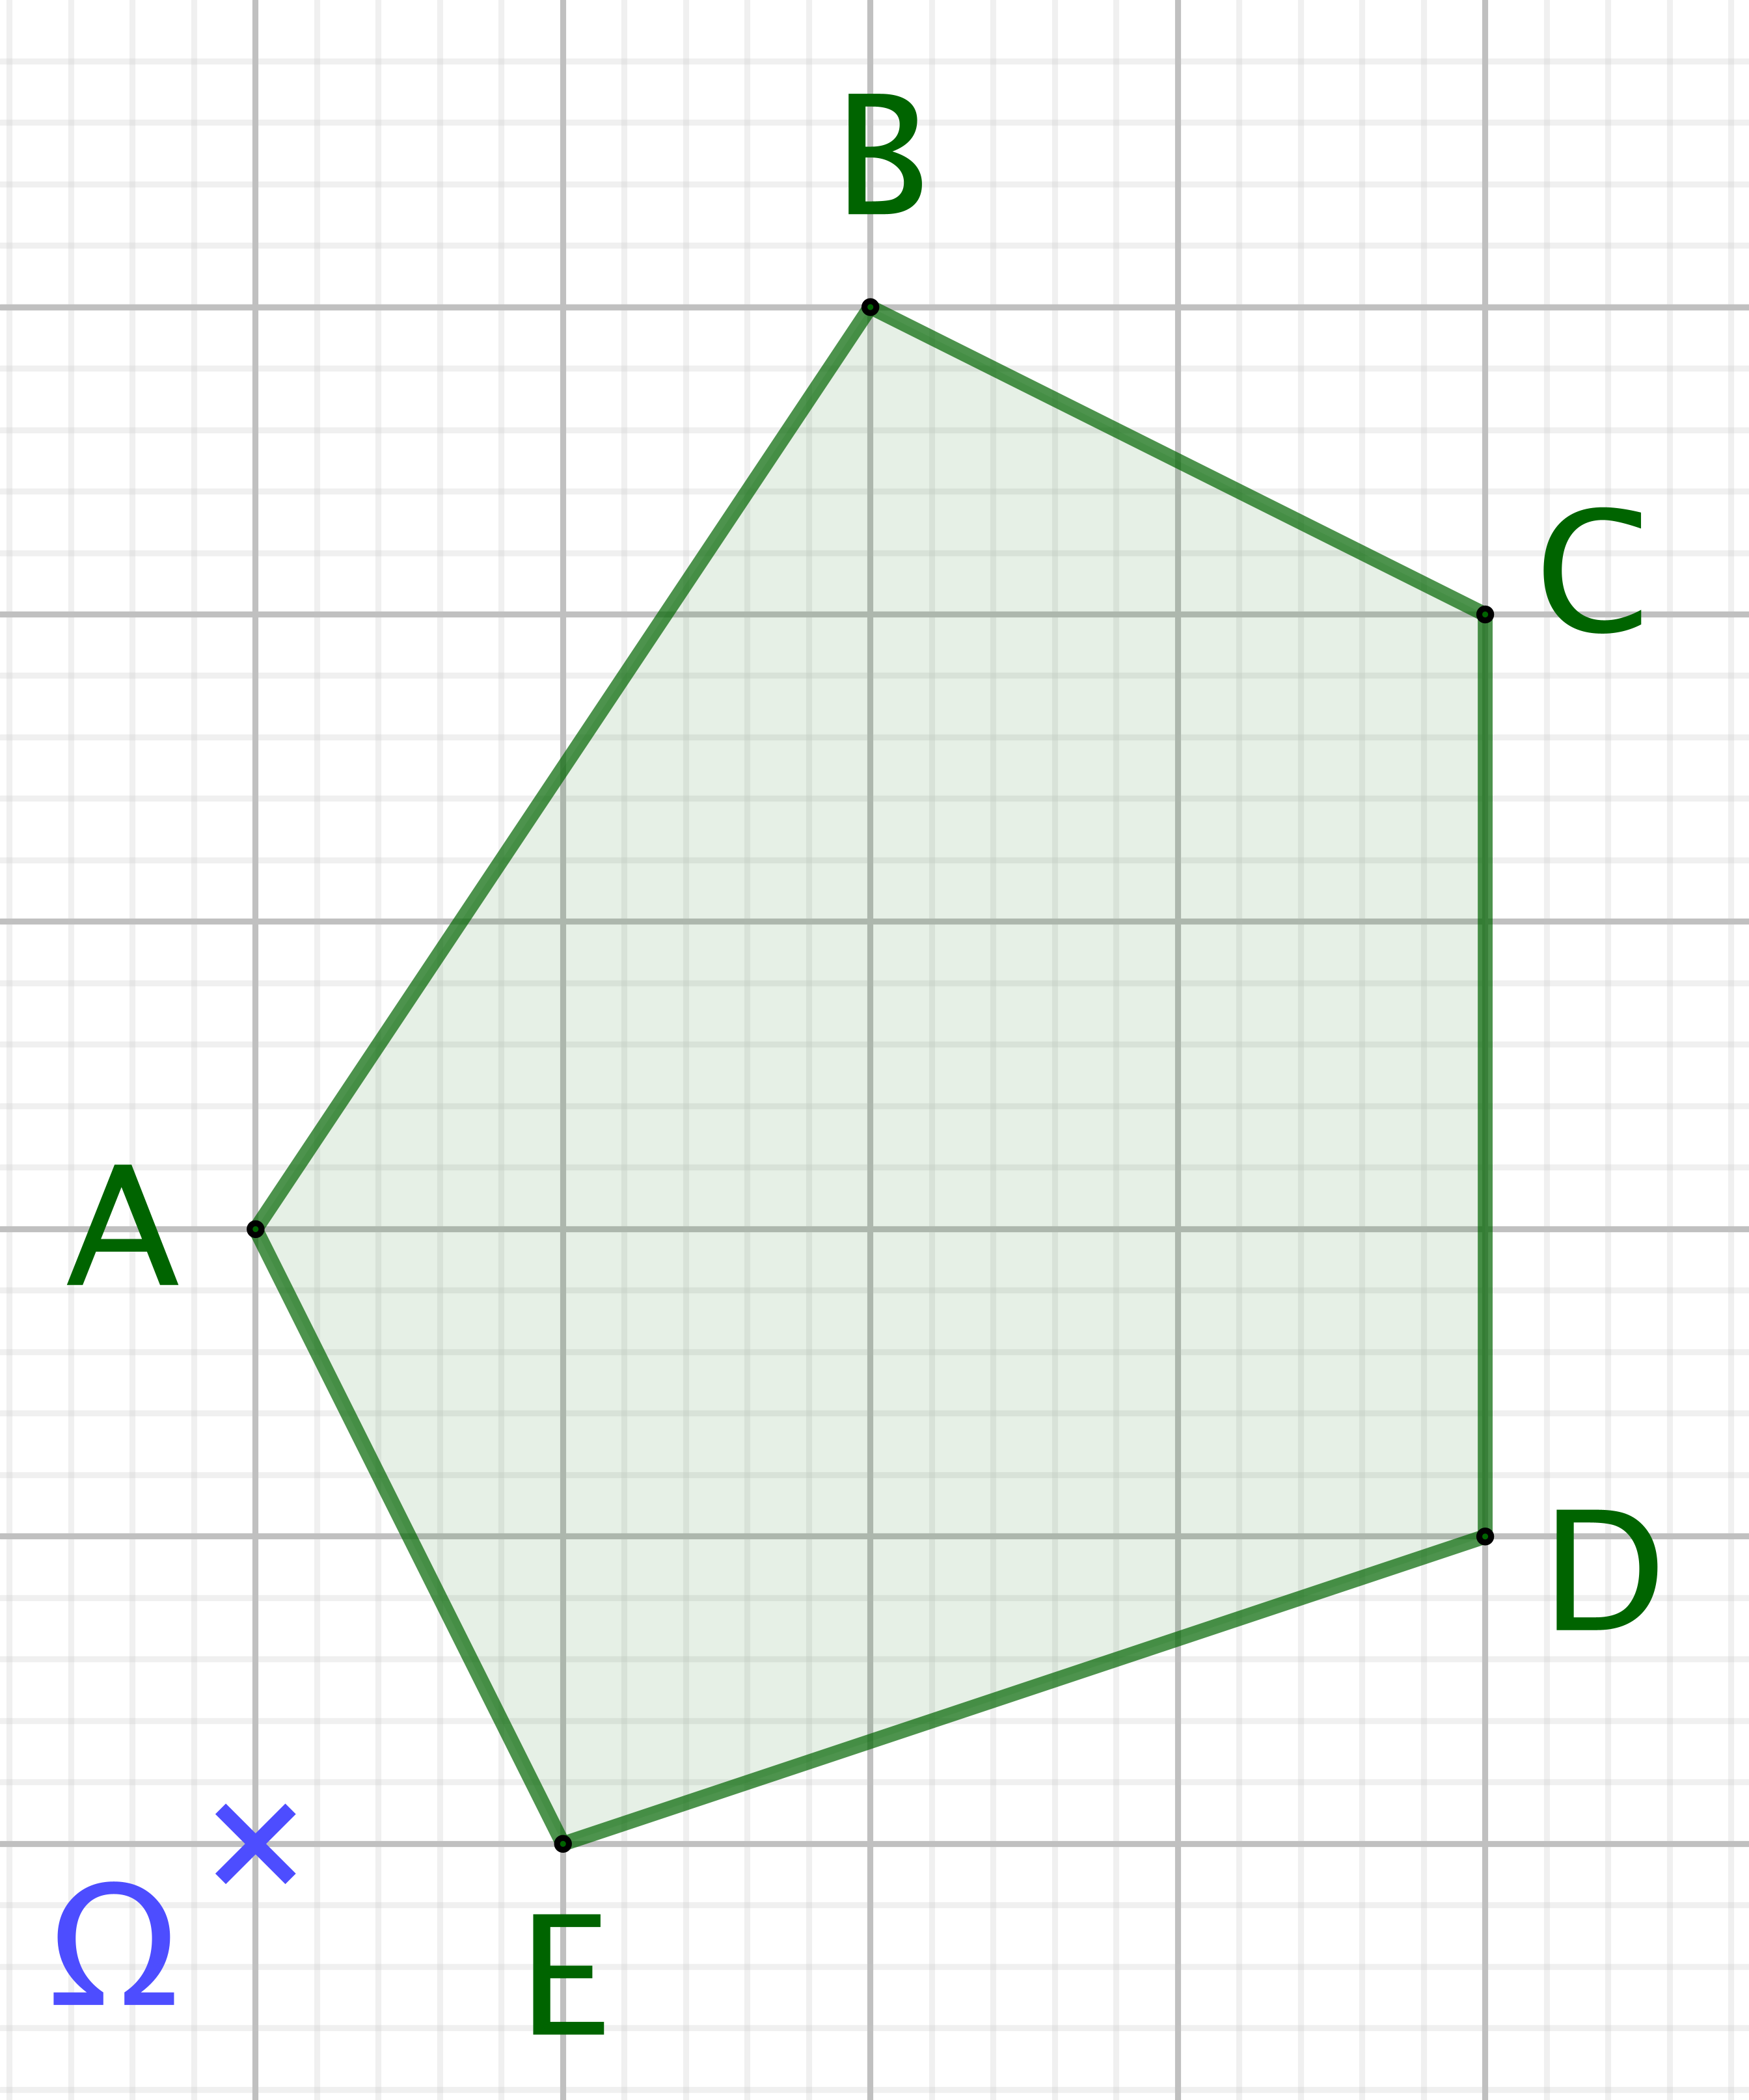
\includegraphics[scale=.4]{content/polygon/sufficient-cond/convex-1.png}
        
       	\smallskip
	
		$\num{14.5} = 4 \cdot 6 - \dfrac{2 \cdot 4 + 2 \cdot 1 + 3 \cdot 2 + 1 \cdot 3}{2}$
    \end{center}

	\columnbreak
	
    \begin{center}
        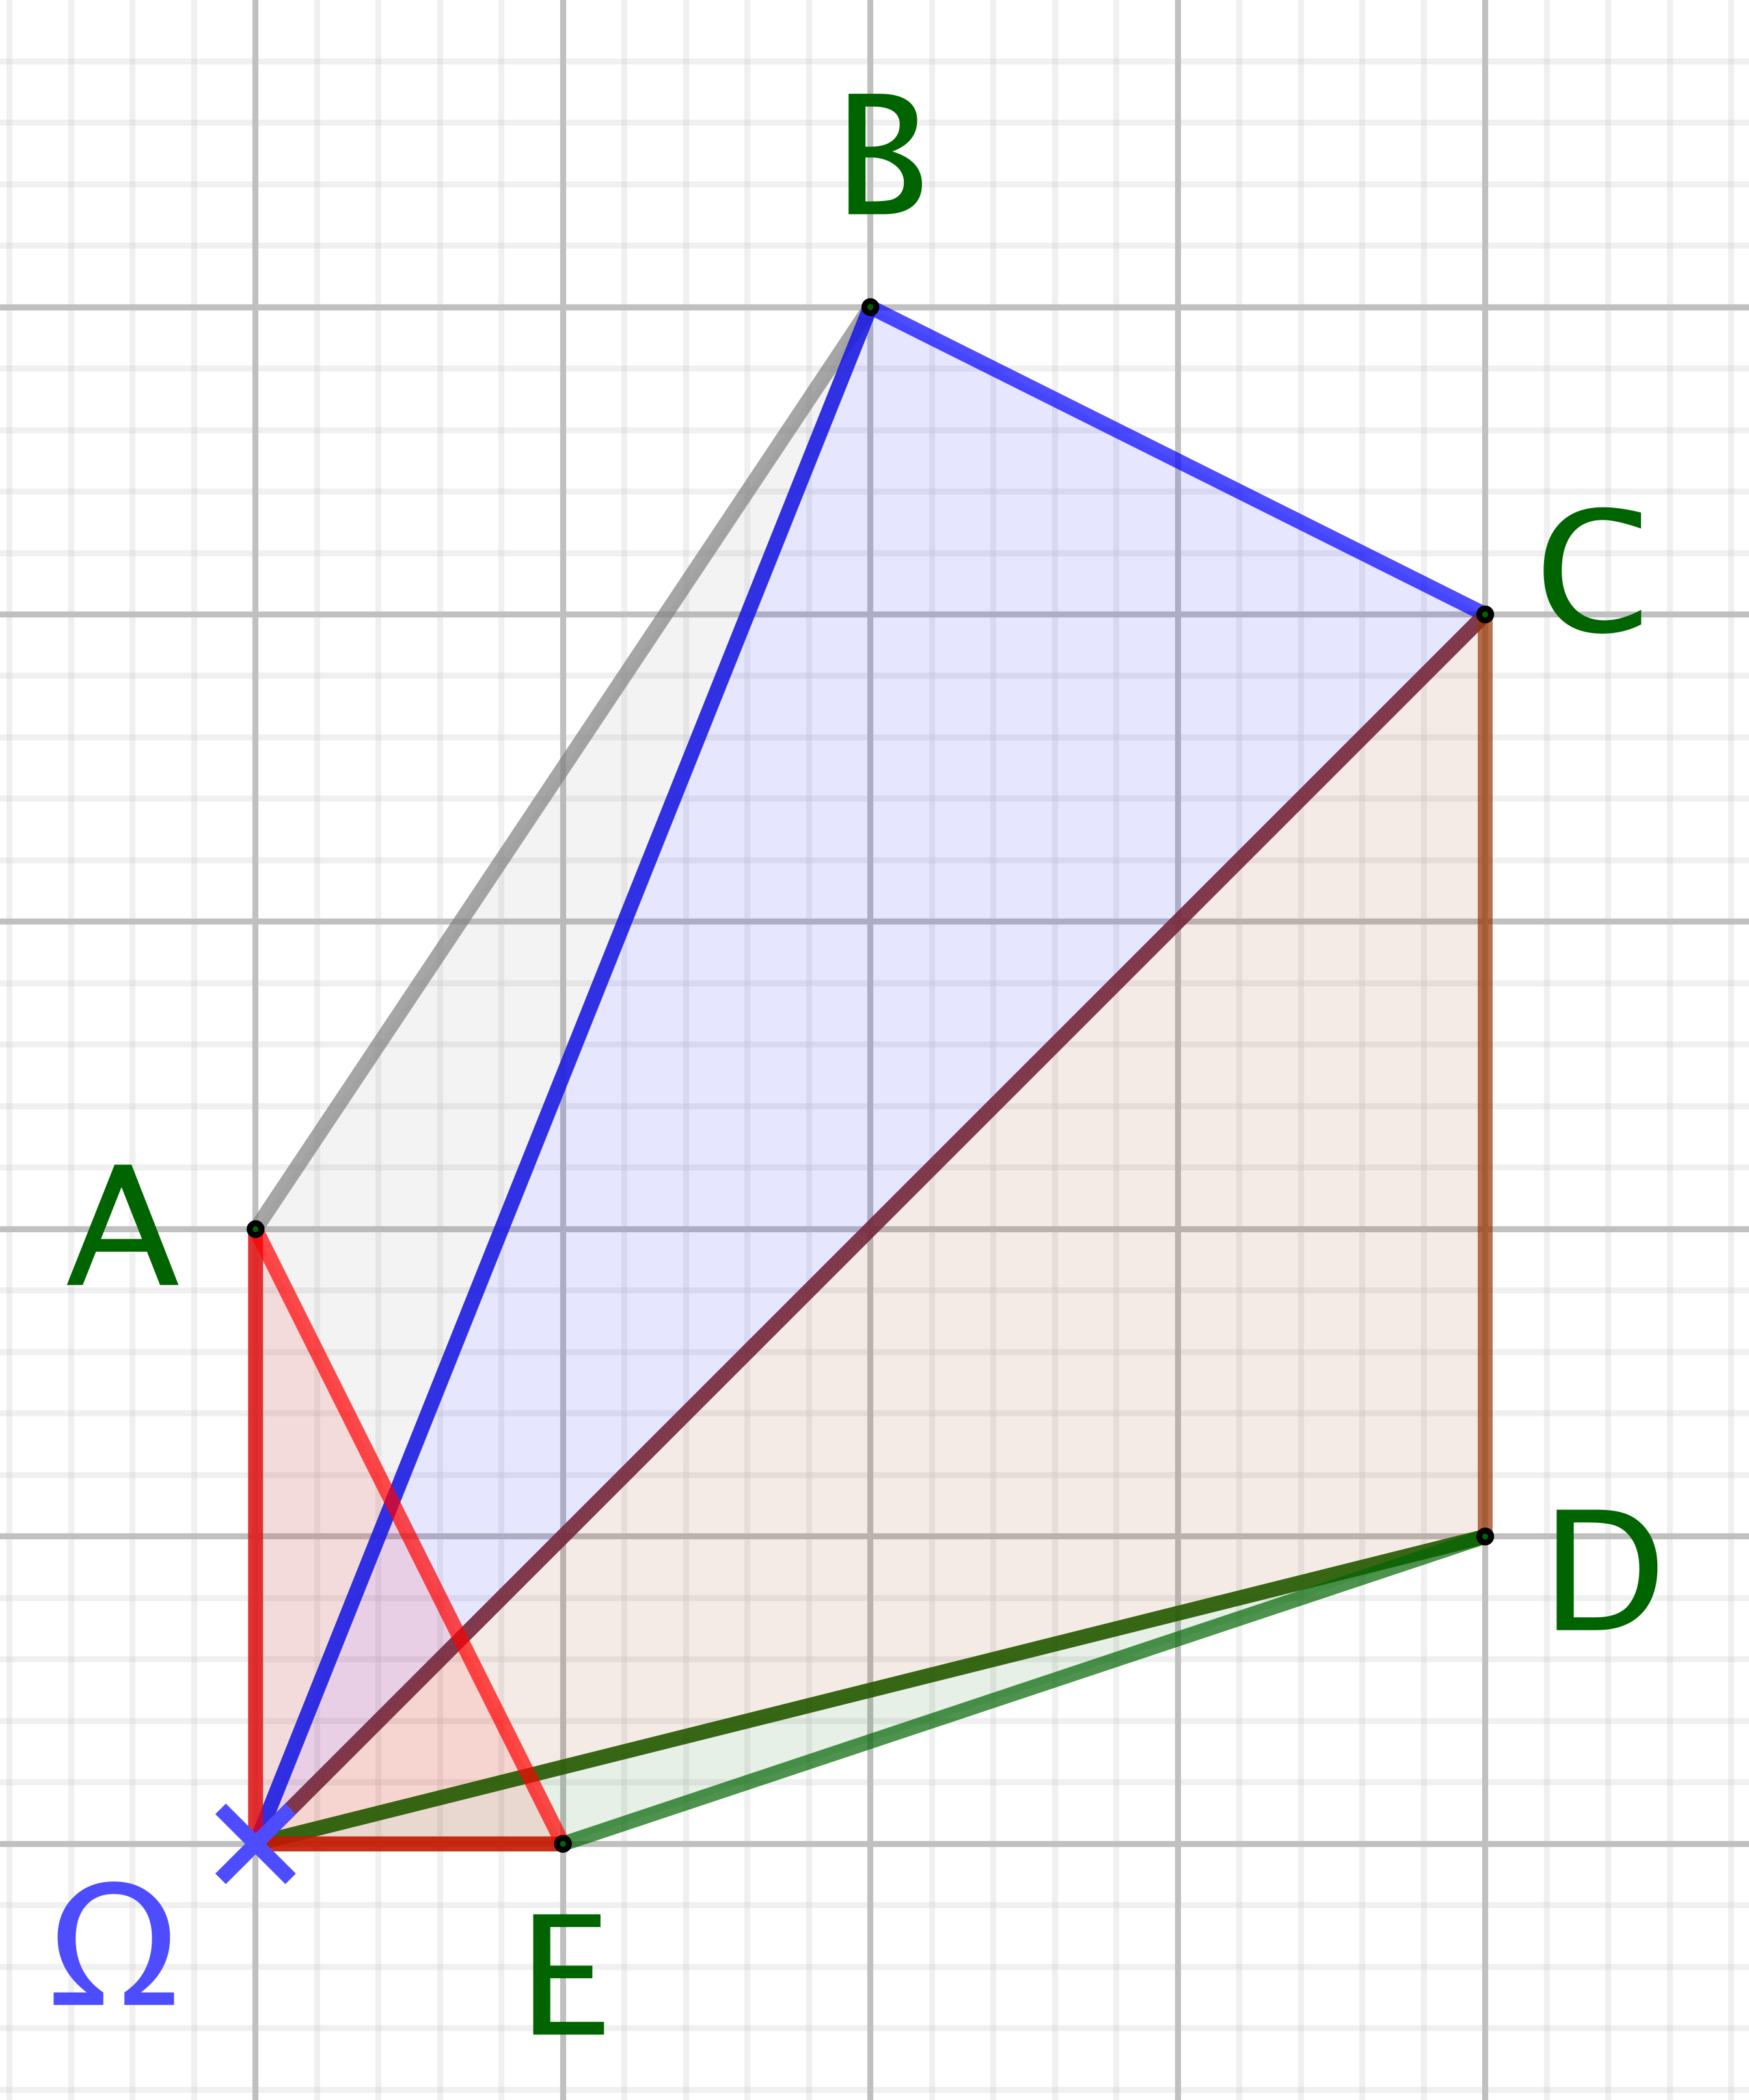
\includegraphics[scale=.4]{content/polygon/sufficient-cond/convex-2.png}
        
       	\smallskip
	
		$\num{14.5} = 2 + 7 + 4 + \num{4.5} - 4 \vphantom{\dfrac22}$
    \end{center}
\end{multicols}


Ce mode de calcul est celui employé par \geogebra\ qui donne une aire de \num{6.5} pour le polygone croisé de la bande dessinée ci-après qui détaille les calculs faits: les aires algébriques représentées en vert sont positives, et celles en rouge négatives.
Nous obtenons un total de $( - \num{6.5})$, soit la valeur fournie par \geogebra\ au signe près.

\newpage

\begin{multicols}{3}
    \small\itshape
    
    \begin{center}
        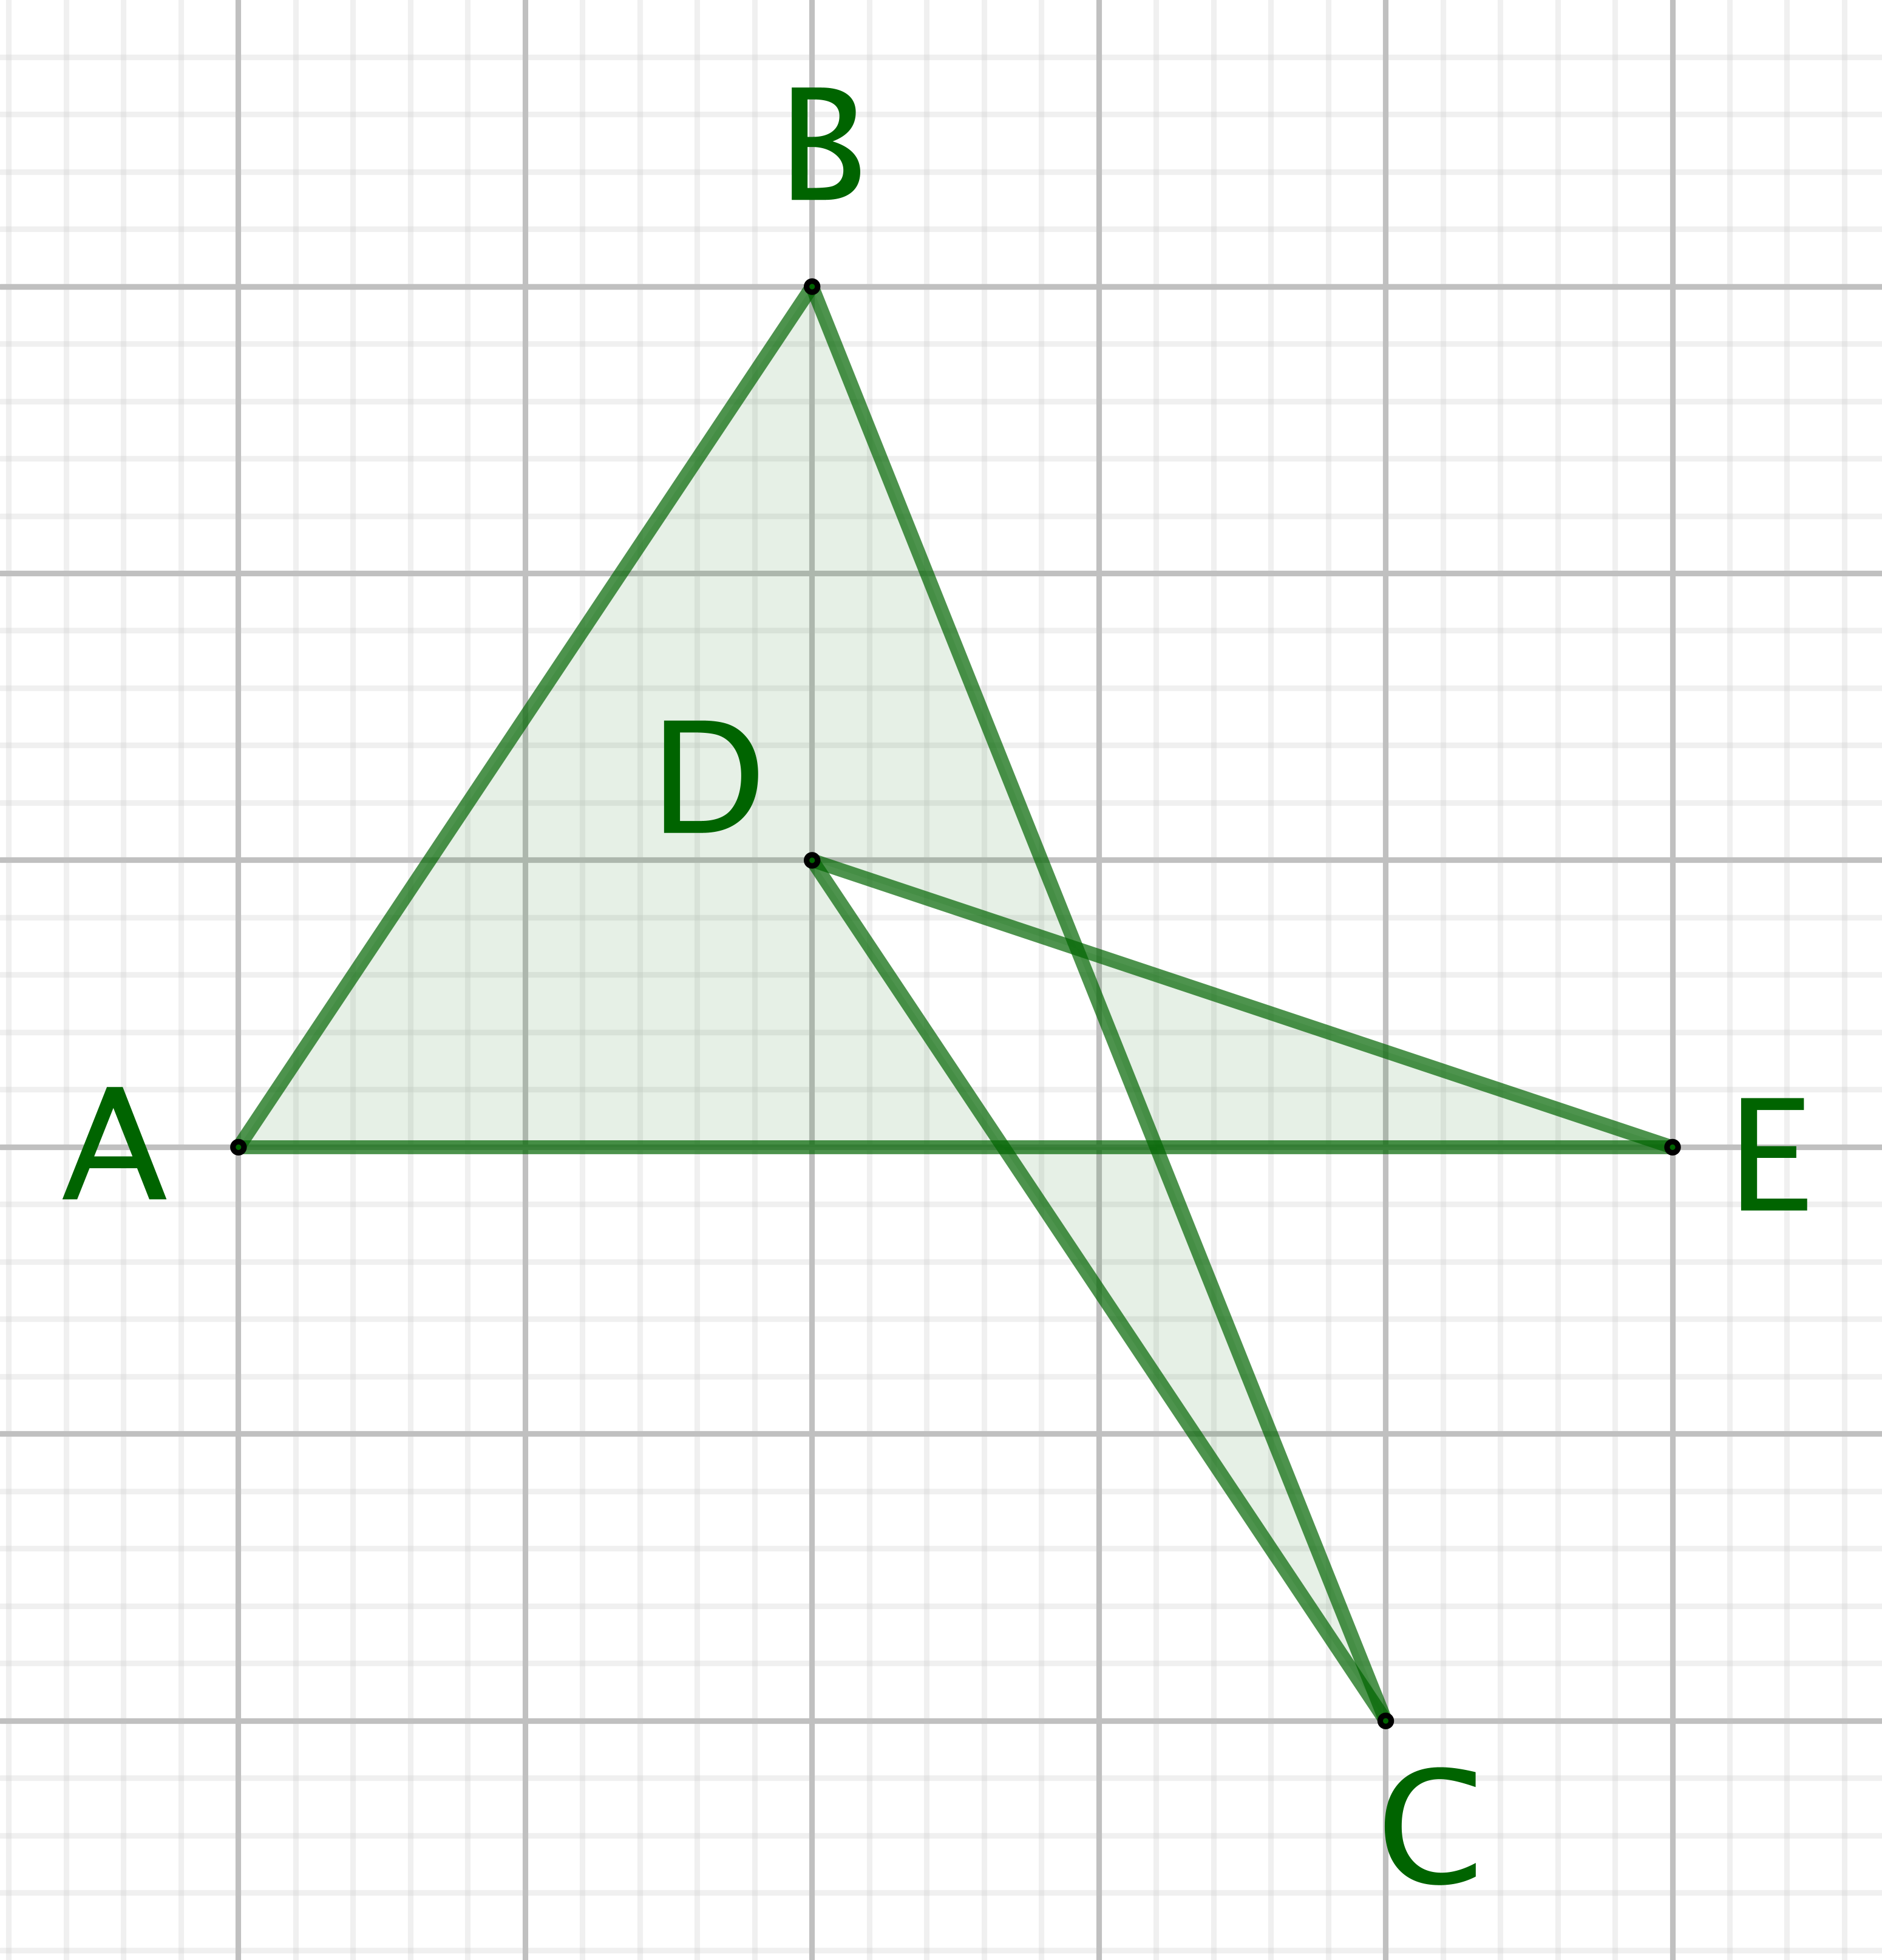
\includegraphics[scale=.4]{content/polygon/sufficient-cond/why.png}
    \end{center}
    
    \foreach \i in {3,1,4,2,5} {
    	\begin{center}
            \includegraphics[scale=.4]{content/polygon/sufficient-cond/why-step-\i.png}
        \end{center}
	}
\end{multicols}


Avant de formaliser ce qui précède, il faut noter que la notion d'aire algébrique est à manier avec prudence lorsqu'on la découvre. 
Si c'est votre cas, que pensez-vous de l'aire algébrique du quadrilatère croisé $ABCD$ ci-dessous qui est un antiparallélogramme très particulier? Réponse en note de bas de page.%
\footnote{
    La réponse est $0$. Comme nous verrons que le choix de $\Omega$ est libre, il suffit de faire les calculs avec $\Omega$ l'intersection des segments $[AD]$ et $[BC]$.
    On peut tout de même donner du sens à ceci. Voici comment. 
    Plongeons-nous dans l'espace. 
    Imaginons une toile rectangulaire rouge sur le dessus, et verte en dessous.
    Tournons de \qty{180}{\degree} verticalement l'un des côtés du rectangle.
    En supposant que la toile soit parfaitement tendue, nous obtenons, vue de dessus, un antiparallélogramme dont l'un des triangles est vert, et l'autre rouge.
    De façon savante, les deux faces ont deux orientations différentes. Nous reparlerons de cette notion par la suite.  
}

\begin{center}
    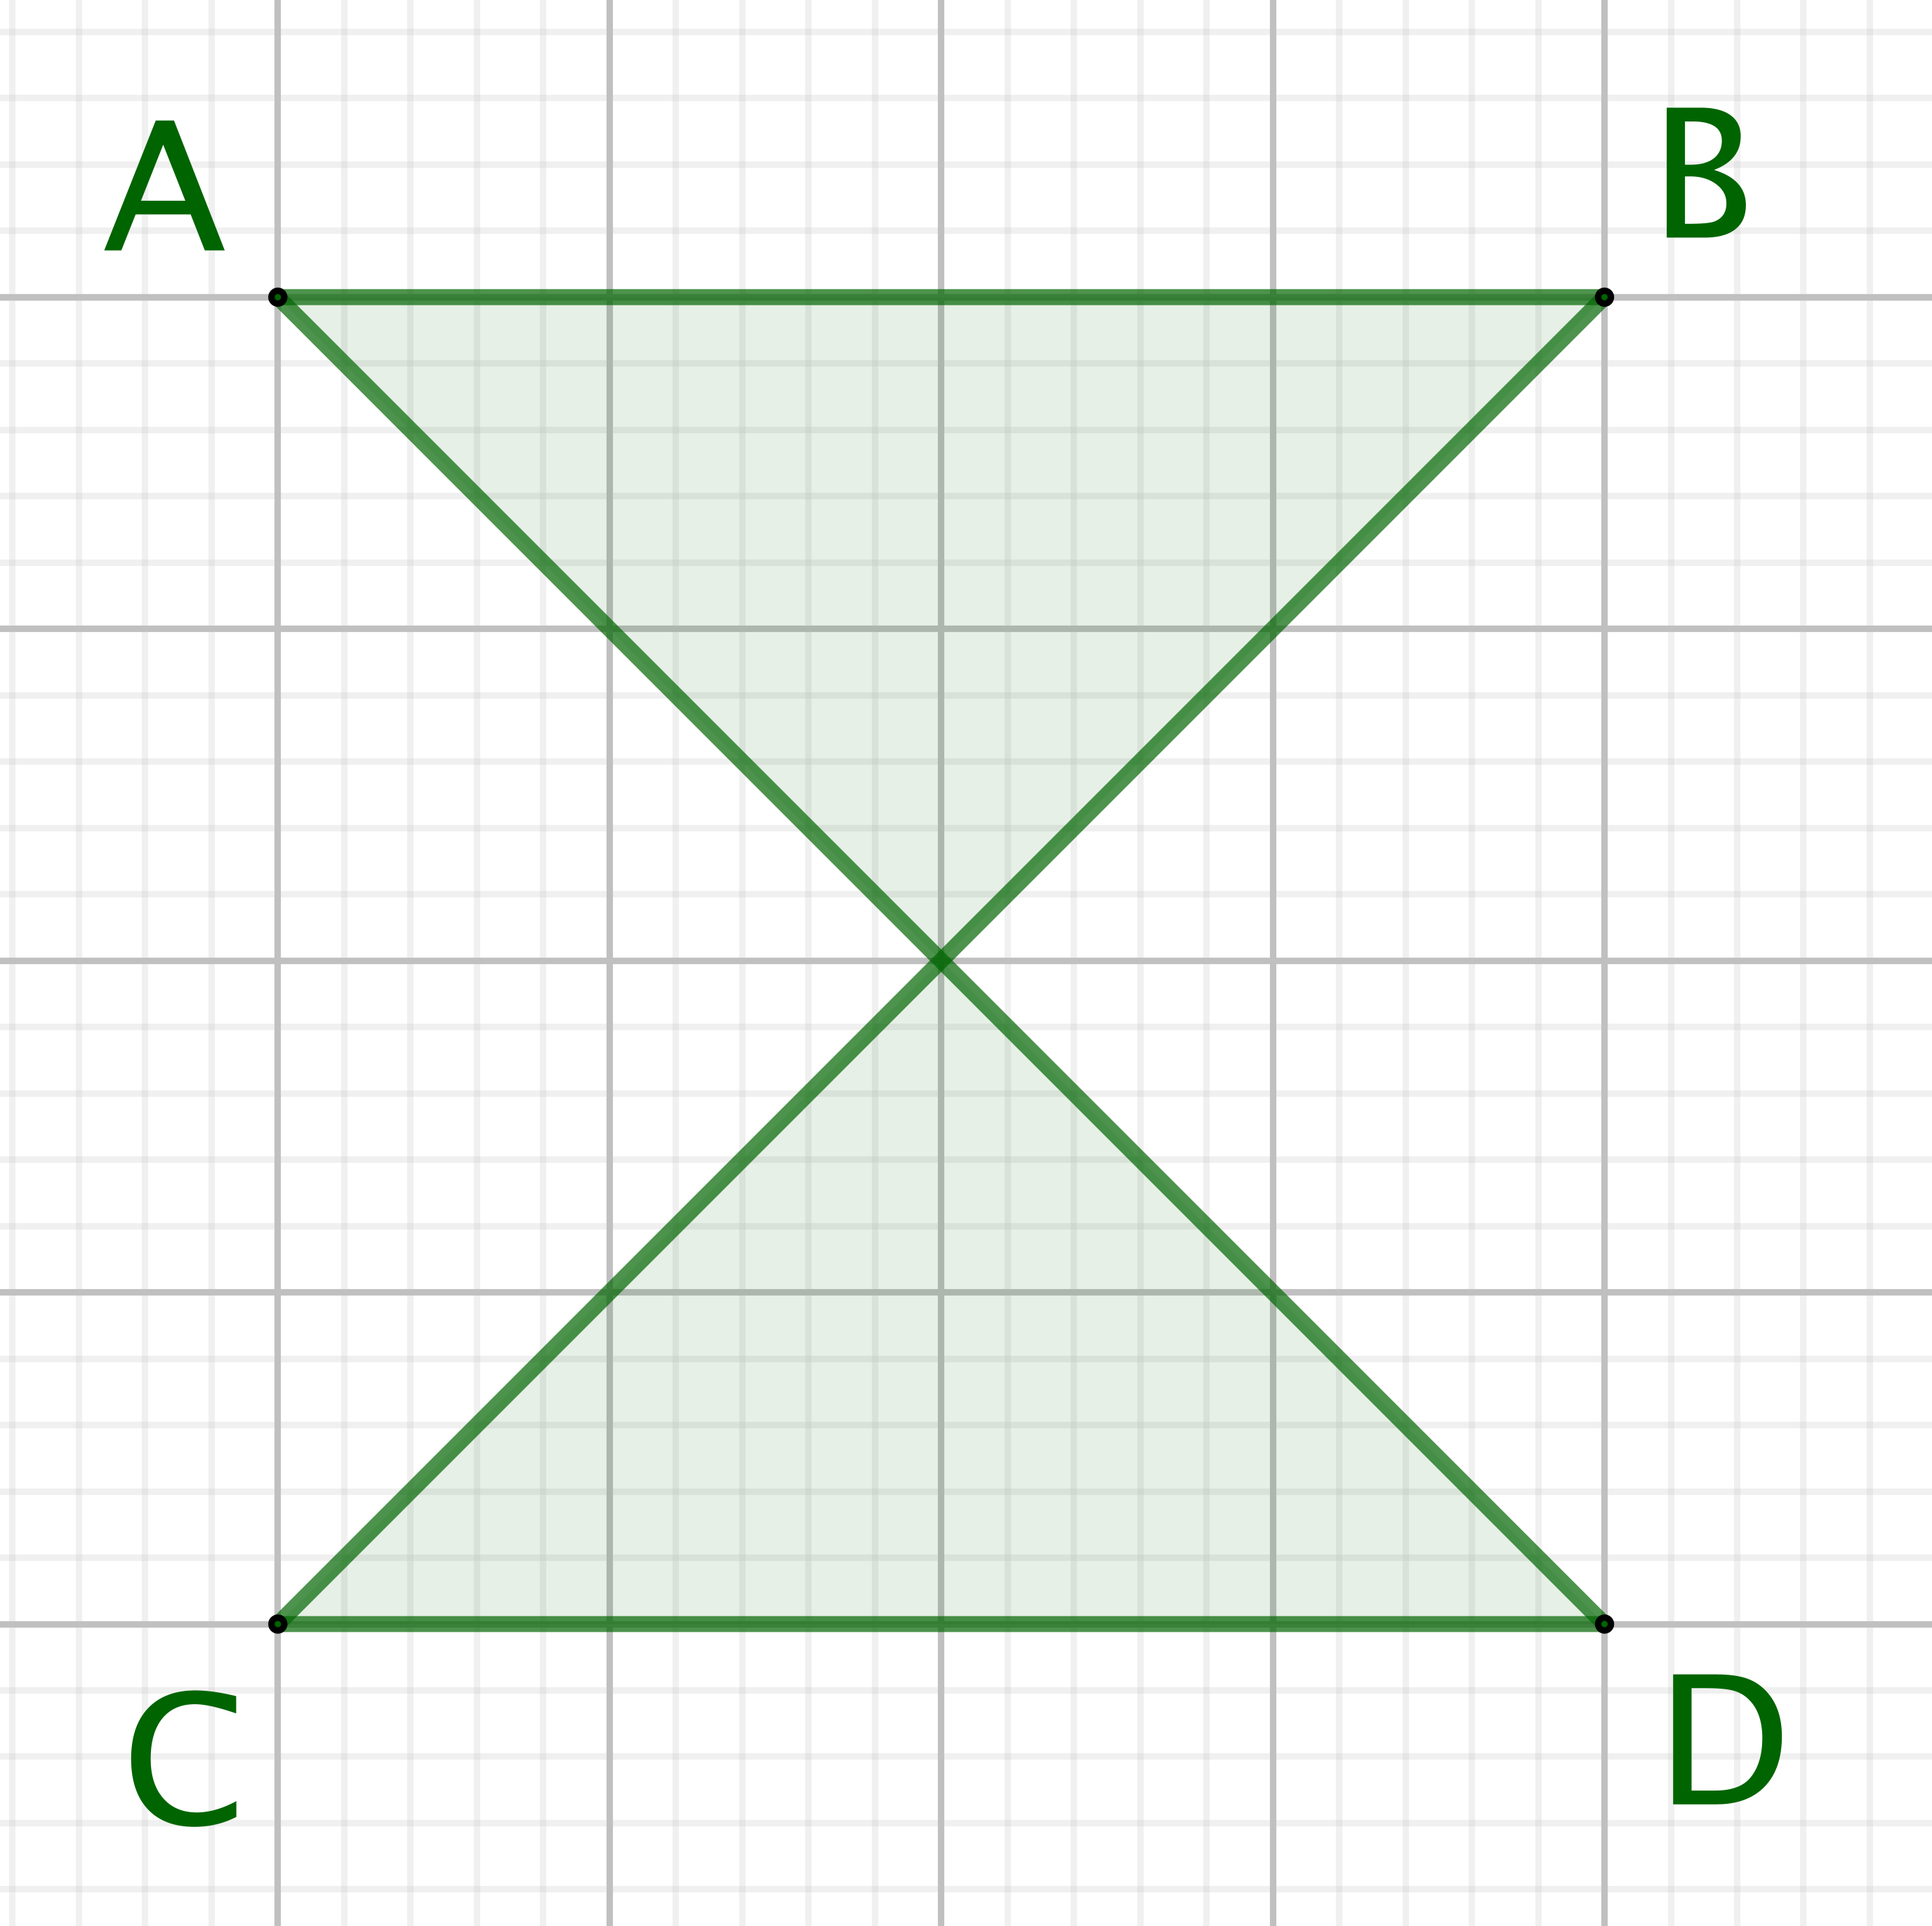
\includegraphics[scale=.4]{content/polygon/sufficient-cond/anti-para.png}
\end{center}


% ----------------------- %


\begin{defi} \label{garea-pt-ct}
    Pour toute \nline\  $\setproba{L} = A_1 A_2 \cdots A_n$, on définit $\big( A^{\,\prime}_i \big)_{i \in \ZZ}$ comme étant $n$-périodique, et vérifiant $A^{\,\prime}_{i} = A_i$ sur $\ZintervalC{1}{n}$.
\end{defi}


% ----------------------- %


\begin{fact} \label{garea-pt-ct}
    Soit $\setproba{L} = A_1 A_2 \cdots A_n$ une \nline.
    La fonction qui à un point $\Omega$ du plan associe 
    $\mu_1^n (\Omega ;\setproba{L}) = \dsum_{i=1}^{n} \det \big( \vect{\Omega A^{\,\prime}_i} , \vect{\Omega A^{\,\prime}_{i+1}} \big)$ est indépendante du point $\Omega$.
    Dans la suite, cette quantité indépendante de $\Omega$ sera notée $\mu_1^n (\setproba{L})$.
\end{fact}


\begin{proof}
    Soit $M$ un autre point du plan.

    \begin{stepcalc}[style=ar*]
        \mu_1^n (\Omega ;\setproba{L})
    \explnext{}
        \dsum_{i=1}^{n} \det \big( \vect{\Omega A^{\,\prime}_i} , \vect{\Omega A^{\,\prime}_{i+1}} \big)
    \explnext*{Cette bonne vieille relation de Chasles.}{}
        \dsum_{i=1}^{n} \det \big( \vect{\Omega M} + \vect{M A^{\,\prime}_i} , \vect{\Omega M} + \vect{M A^{\,\prime}_{i+1}} \big)
    \explnext{}
        \dsum_{i=1}^{n} \Big[
            \det \big( \vect{\Omega M} , \vect{\Omega M} \big)
            +
            \det \big( \vect{\Omega M} , \vect{M A^{\,\prime}_{i+1}} \big)
            +
            \det \big( \vect{M A^{\,\prime}_i} , \vect{\Omega M} \big)
            +
            \det \big( \vect{M A^{\,\prime}_i} , \vect{M A^{\,\prime}_{i+1}} \big)
        \Big]
    \explnext{}
        \dsum_{i=1}^{n} \det \big( \vect{\Omega M} , \vect{M A^{\,\prime}_{i+1}} \big)
        +
        \dsum_{i=1}^{n} \det \big( \vect{M A^{\,\prime}_i} , \vect{\Omega M} \big)
        +
        \mu_1^n (M ; \setproba{L})
    \explnext{}
        \mu_1^n (M ; \setproba{L})
        +
        \dsum_{i=2}^{n+1} \det \big( \vect{\Omega M} , \vect{M A^{\,\prime}_{i}} \big)
        -
        \dsum_{i=1}^{n} \det \big( \vect{\Omega M} , \vect{M A^{\,\prime}_i} \big)
    \explnext{}
        \mu_1^n (M ; \setproba{L})
        +
        \det \big( \vect{\Omega M} , \vect{M A^{\,\prime}_{n+1}} \big)
        -
        \det \big( \vect{\Omega M} , \vect{M A^{\,\prime}_1} \big)
    \explnext*{$A^{\,\prime}_{n+1} = A^{\,\prime}_1$}{}
        \mu_1^n (M ; \setproba{L})
    \end{stepcalc}
    
    \null\vspace{-3.5ex}
\end{proof}
    
    
% ----------------------- %


\begin{fact} \label{nline-shift-inva}
    Soit $\setproba{L} = A_1 A_2 \cdots A_n$ une \nline.
    Pour $k \in \ZintervalC{1}{n}$, 
    la \nline\ $\setproba{L}_j = B_1 B_2 \cdots B_n$, où $B_i = A^{\,\prime}_{k+i-1}$,
    vérifie
    $\mu_1^n (\setproba{L}) = \mu_1^n (\setproba{L}_k)$.
    Dans la suite, cette quantité commune sera notée $\mu (\setproba{L})$.
\end{fact}


\begin{proof}
    Il suffit de s'adonner à un petit jeu sur les indices de sommation.
\end{proof}
    
    
% ----------------------- %


\begin{fact} \label{nline-rota-inva}
    Soit 
    $\setproba{L} = A_1 A_2 \cdots A_n$ une \nline. 
    La \nline\ $\setproba{L}^{\mathrm{op}} = B_1 B_2 \cdots B_n$, où $B_i =  A_{n + 1 - i}$,
    vérifie
    $\mu(\setproba{L}^{\mathrm{op}}) = {} - \mu(\setproba{L})$.
\end{fact}


\begin{proof}
    Soit $\Omega$ un point quelconque du plan.

    \begin{stepcalc}[style=ar*]
        \mu(\setproba{L}^{\mathrm{op}})
    \explnext{}
        \dsum_{i=1}^{n} \det \big( \vect{\Omega B^{\,\prime}_i} , \vect{\Omega B^{\,\prime}_{i+1}} \big)
    \explnext{}
        \dsum_{i=1}^{n} \det \big( \vect{\Omega A^{\,\prime}_{n + 1 - i}} , \vect{\Omega A^{\,\prime}_{n - i}} \big)
    \explnext{}
        \dsum_{j=0}^{n-1} \det \big( \vect{\Omega A^{\,\prime}_{j + 1}} , \vect{\Omega A^{\,\prime}_j} \big)
    \explnext*{$A^{\,\prime}_0 = A^{\,\prime}_n$ et $A^{\,\prime}_1 = A^{\,\prime}_{n+1}$}{}
        \dsum_{j=1}^{n} \det \big( \vect{\Omega A^{\,\prime}_{j + 1}} , \vect{\Omega A^{\,\prime}_j} \big)
    \explnext{}
        {} - \dsum_{j=1}^{n} \det \big( \vect{\Omega A^{\,\prime}_j} ,  \vect{\Omega A^{\,\prime}_{j + 1}} \big)
    \explnext{}
        {} - \mu(\setproba{L})
    \end{stepcalc}
    
    \null\vspace{-3.5ex}
\end{proof}
    
    
% ----------------------- %


\begin{fact}
    Soit 
    $\setproba{L} = A_1 A_2 \cdots A_n$ une \nline.
    La quantité $\frac12 \abs{\mu(\setproba{L})}$ ne dépend ni du sens de parcours de $\setproba{L}$, ni du point de départ choisi.%
    \footnote{
        Le lecteur pardonnera les abus de langage utilisés.
    }
    Elle sera notée $\garea{\setproba{L}}$, et nommée \og \emph{aire généralisée} \fg\ de la \nline\ $\setproba{L}$.
\end{fact}


\begin{proof}
    C'est une synthèse des faits \ref{nline-shift-inva} et \ref{nline-rota-inva}.
\end{proof}
    
    
% ----------------------- %


Pour notre démonstration finale, nous aurons besoin de savoir que $\garea{\setproba{P}} = \area{\setproba{P}}$ pour tout \ngone\ $\setproba{P}$.%
\footnote{
	Nous obtenons ainsi la généralisation de l'aire géométrique usuelle au cas des polygones croisés.
}
Ceci est évident dans le cas convexe, car il suffit de choisir l'isobarycentre $G$ de $A_1$, $A_2$, ..., $A_n$ pour le calcul de $\garea{\setproba{P}}$: en effet, avec ce choix, tous les déterminants $\det \big( \vect{G A^{\,\prime}_i} , \vect{G A^{\,\prime}_{i+1}} \big)$ ont le même signe.
Dans le cas non-convexe, les choses se compliquent, car nous ne maîtrisons plus les signes des déterminants. 



???
La présence de la valeur absolue nous demande de connaître mieux le signe

    
    
% ----------------------- %


\begin{fact}
    Pour tout \ngone\ $\setproba{P}$, nous avons: $\garea{\setproba{P}} = \area{\setproba{P}}$.
\end{fact}


\begin{proof}
    Le théorème de triangulation affirme que tout \ngone\ est triangulable comme dans l'exemple très basique suivant qui laisse envisager une démonstration par récurrence en retirant l'un des triangles ayant deux côtés correspondant à deux côtés consécutifs du \ngone\ (pour peu qu'un tel triangle existe toujours).

    
    \begin{multicols}{3}
        \small\itshape
        \begin{center}
            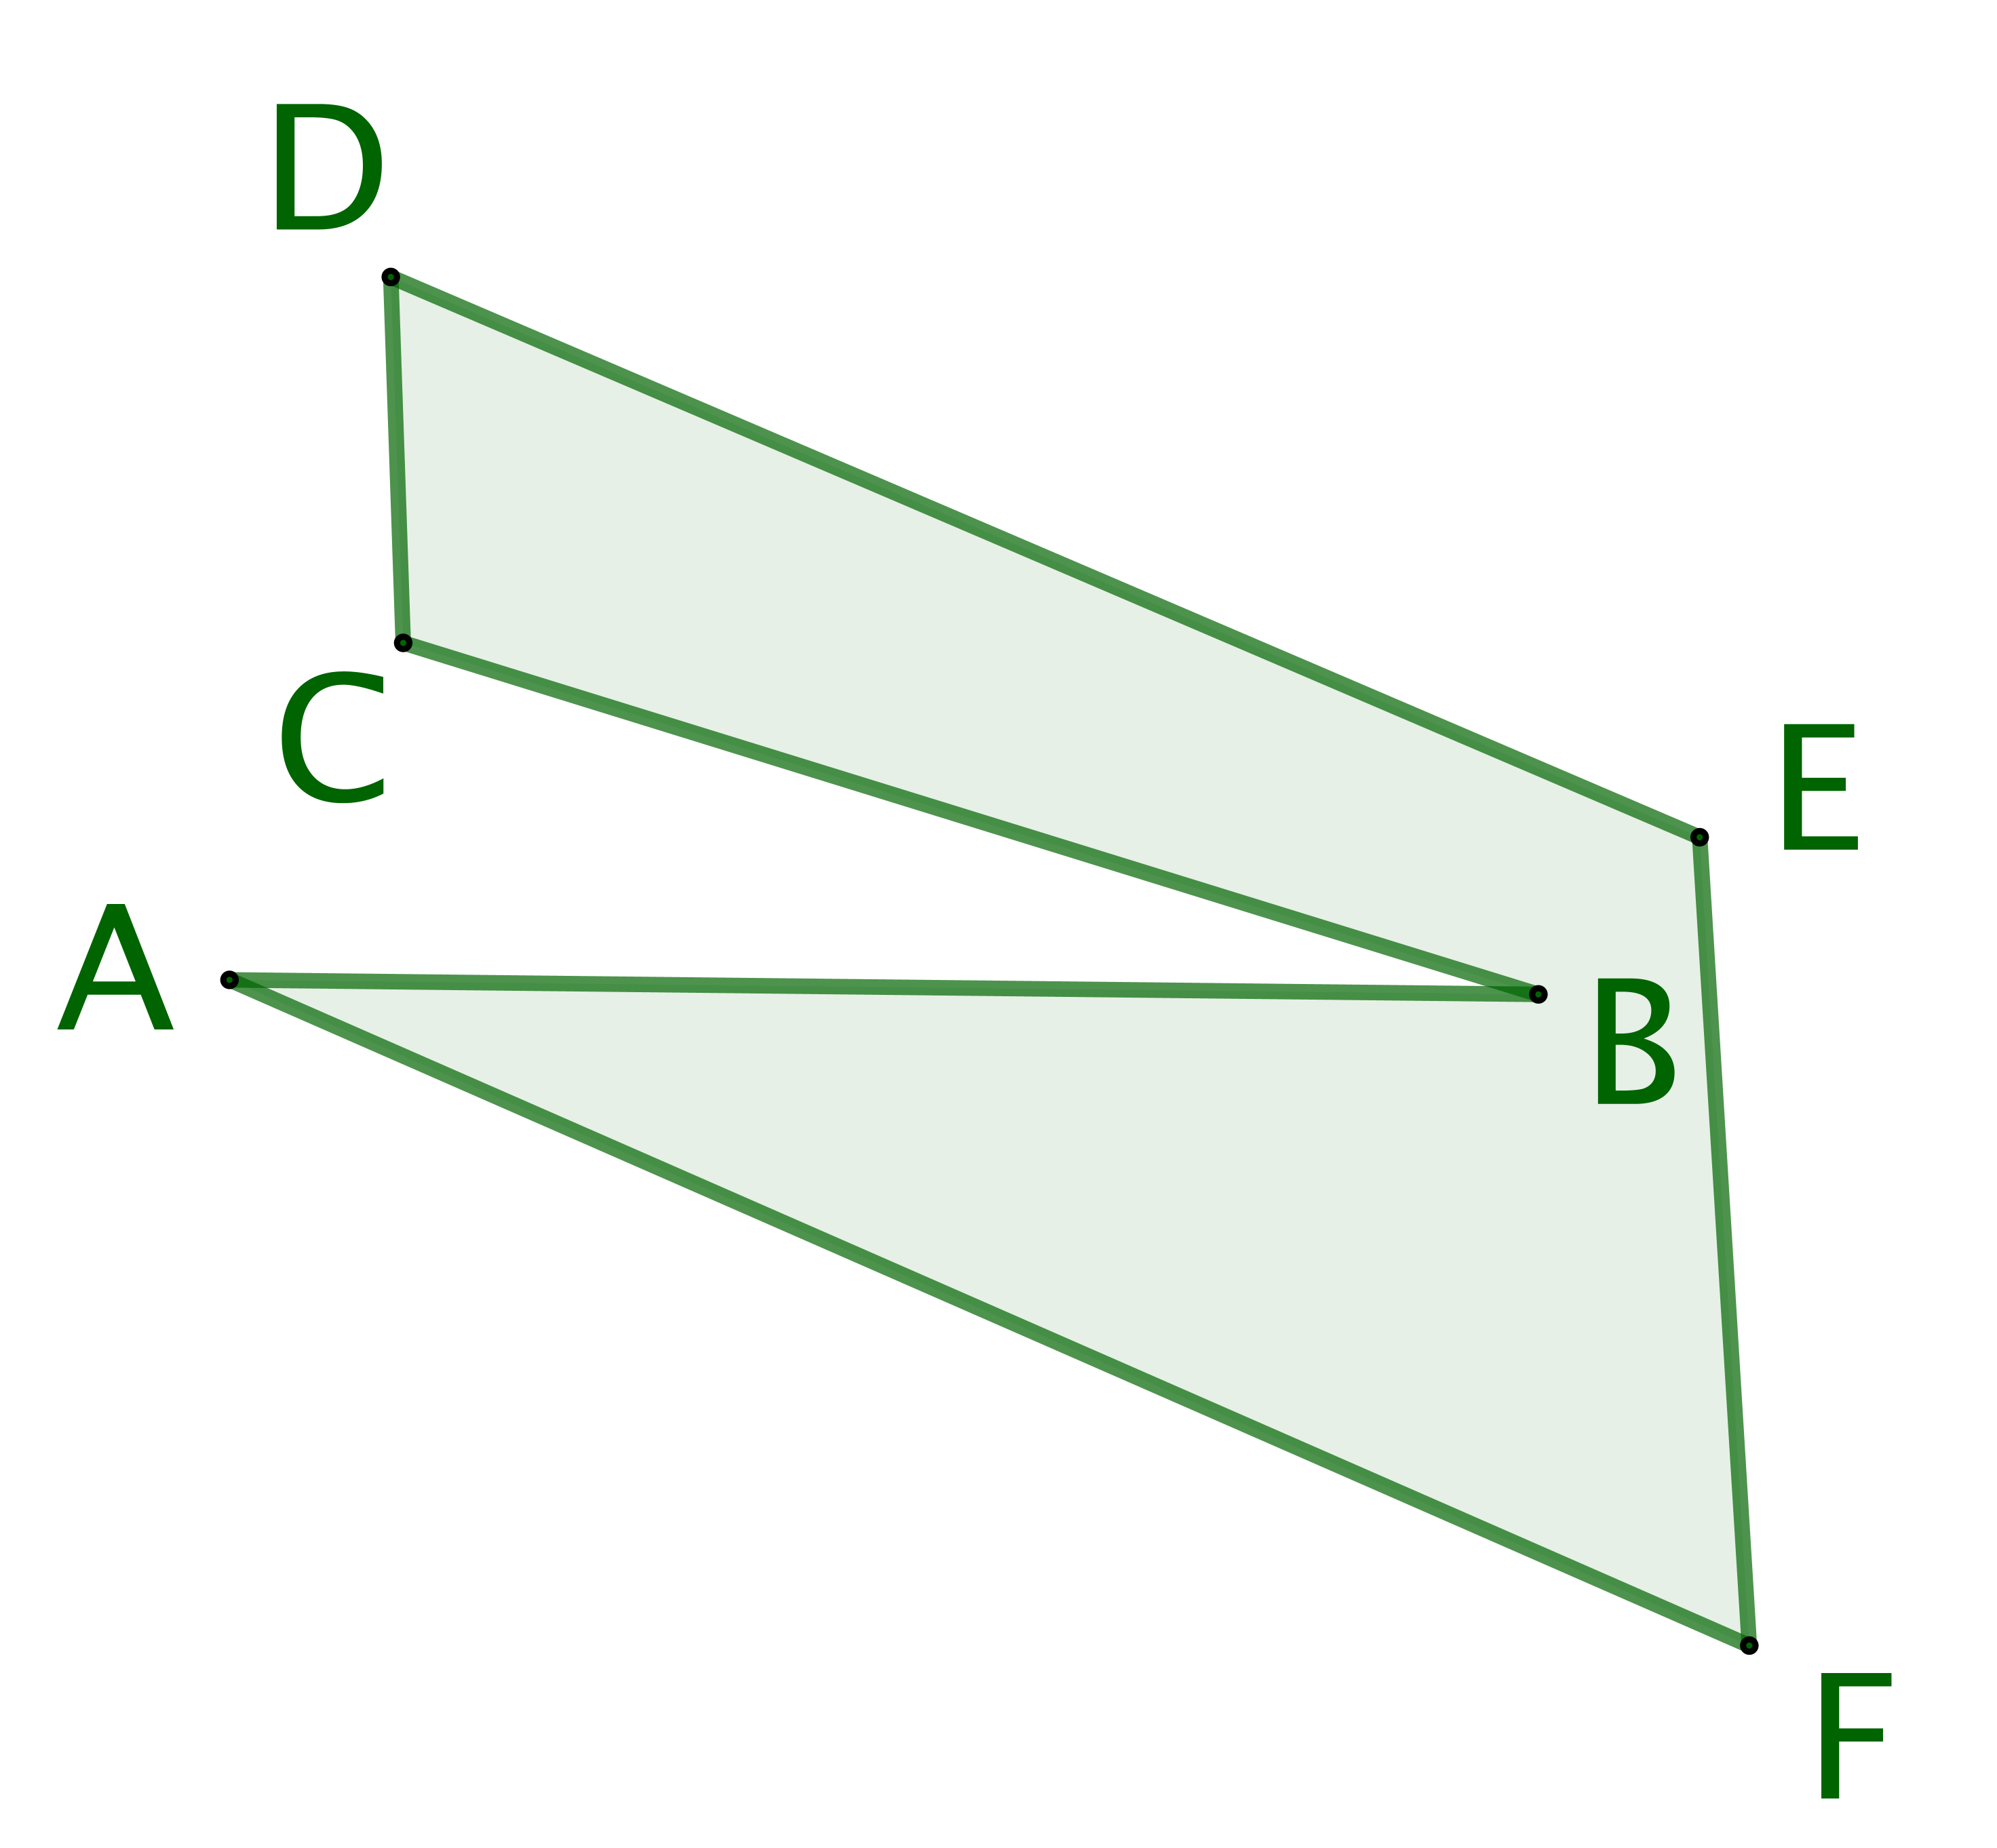
\includegraphics[scale=.4]{content/polygon/sufficient-cond/triangulation-1.png}
        
            \smallskip
            Un \ngone\ nu.
        \end{center}

    
        \begin{center}
            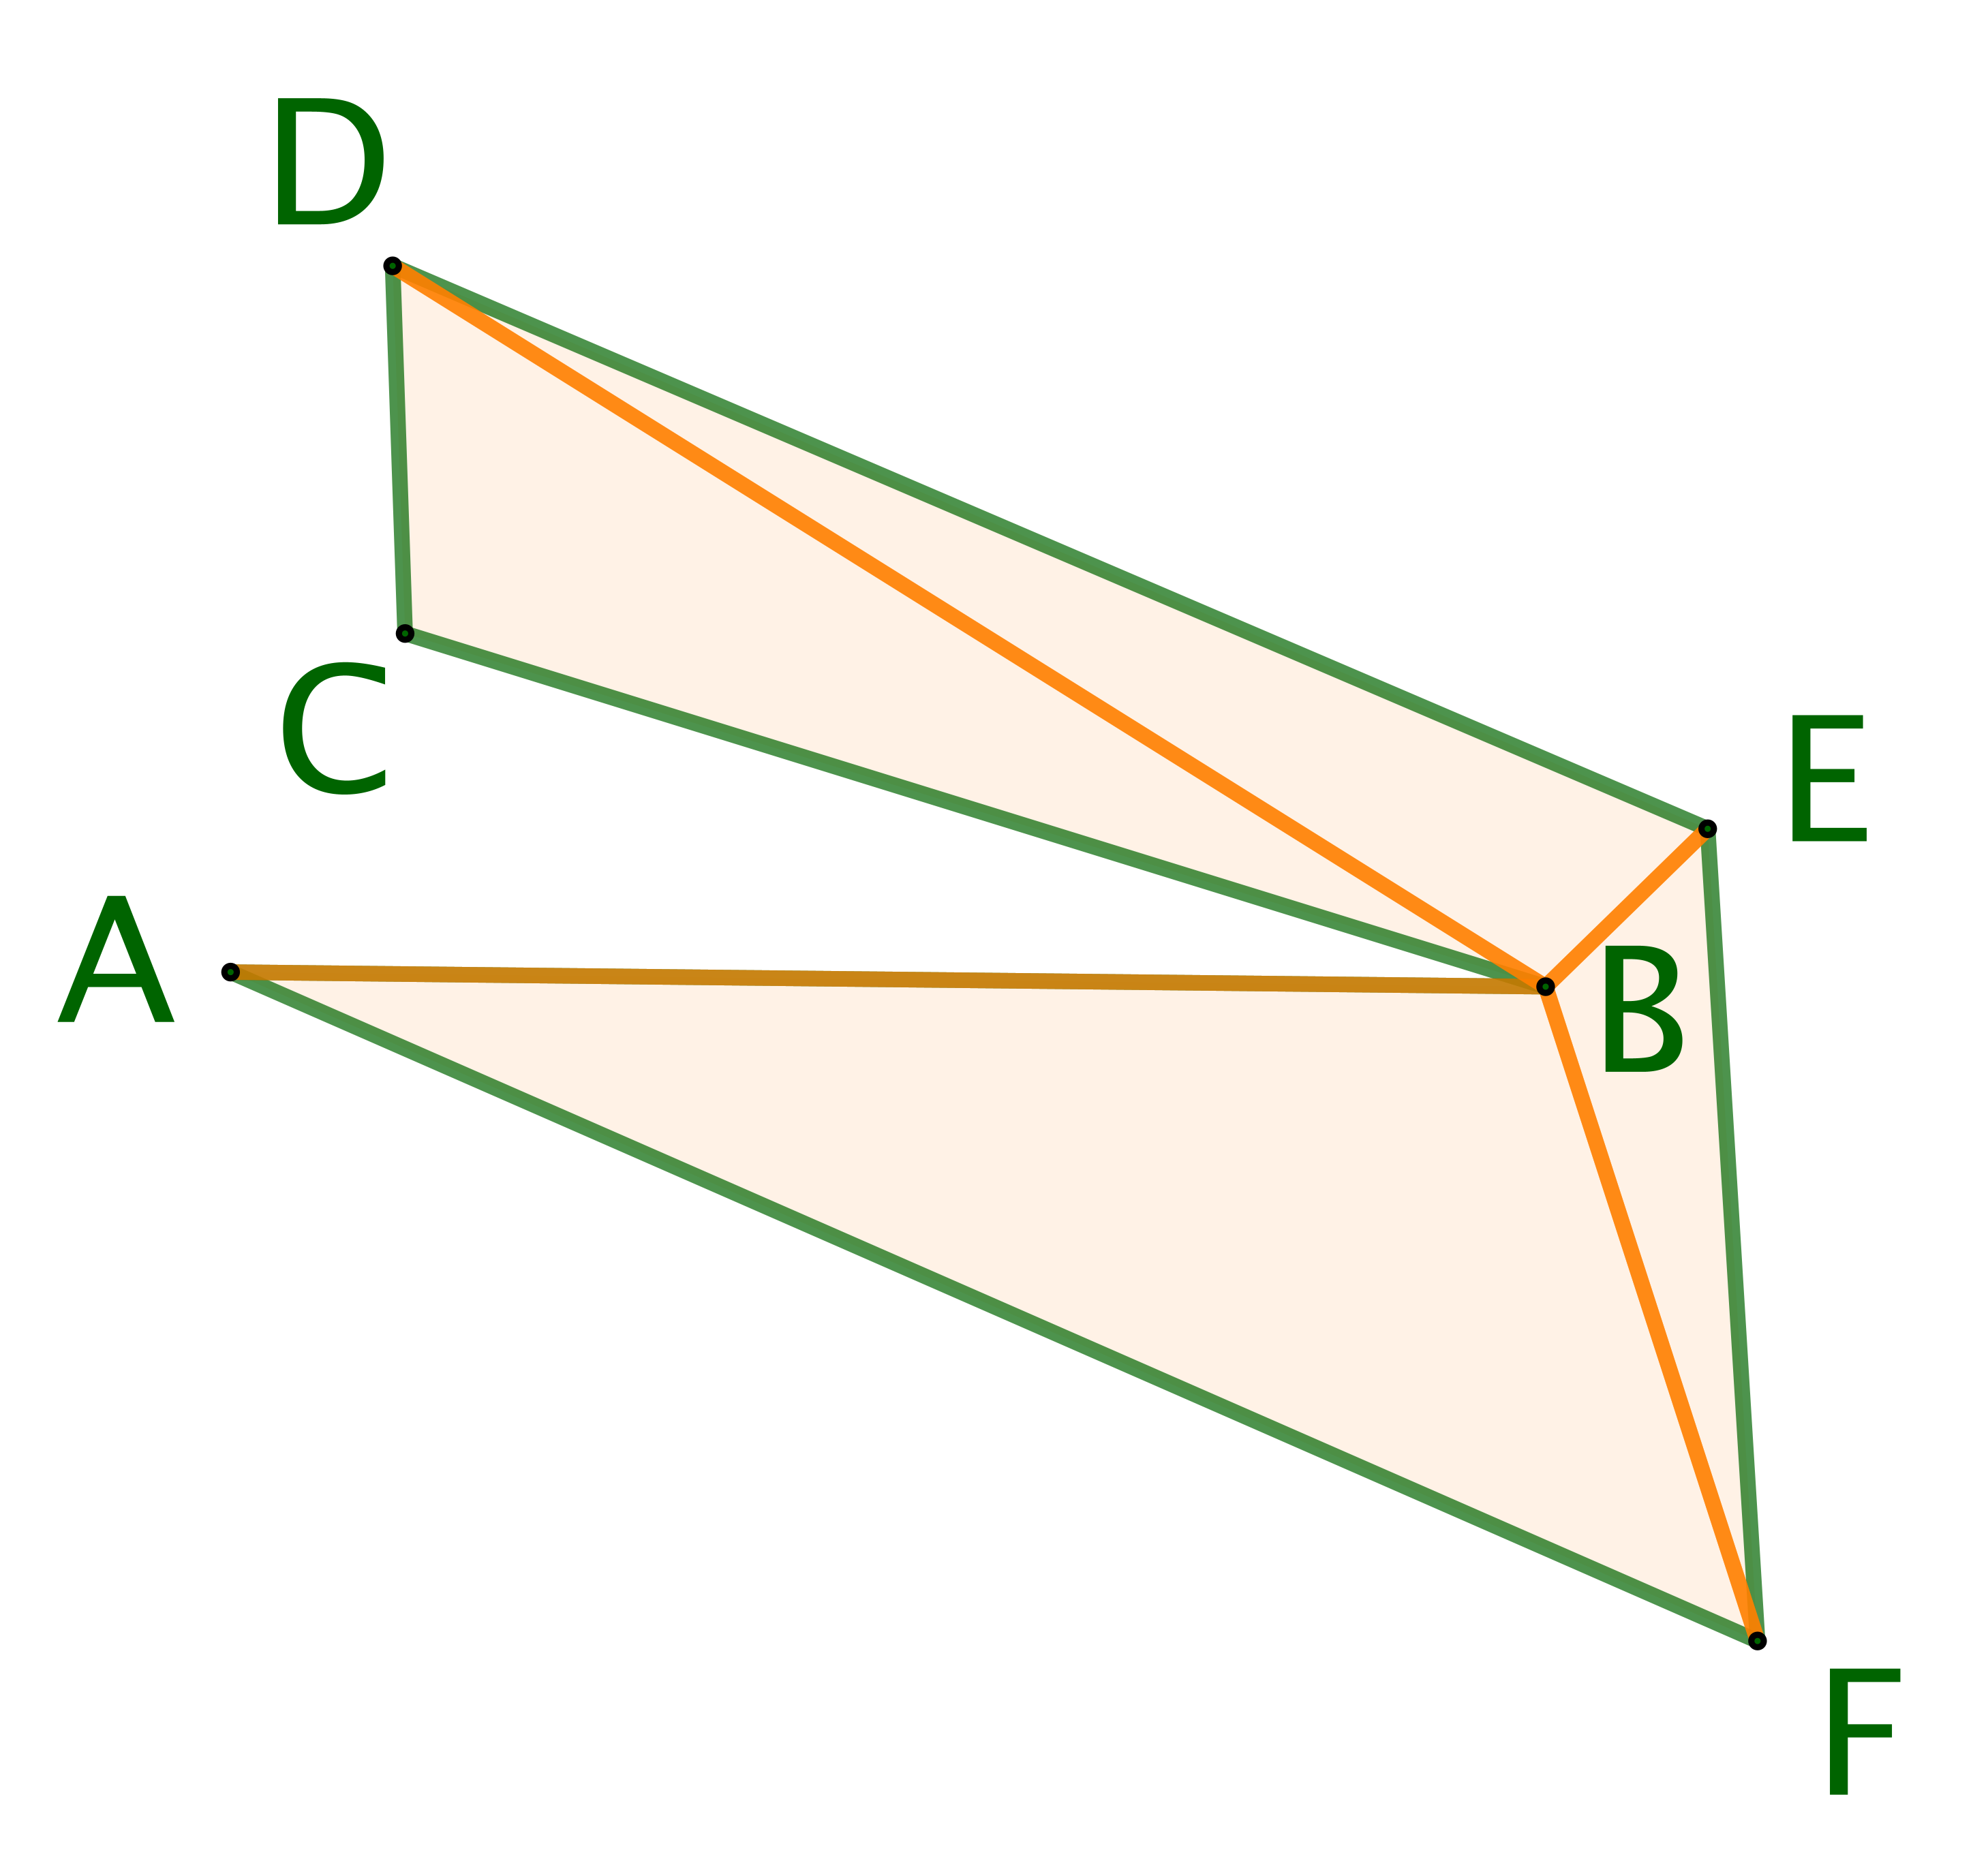
\includegraphics[scale=.4]{content/polygon/sufficient-cond/triangulation-2.png}
        
            \smallskip
            Le \ngone\ triangulé.
        \end{center}

    
        \begin{center}
            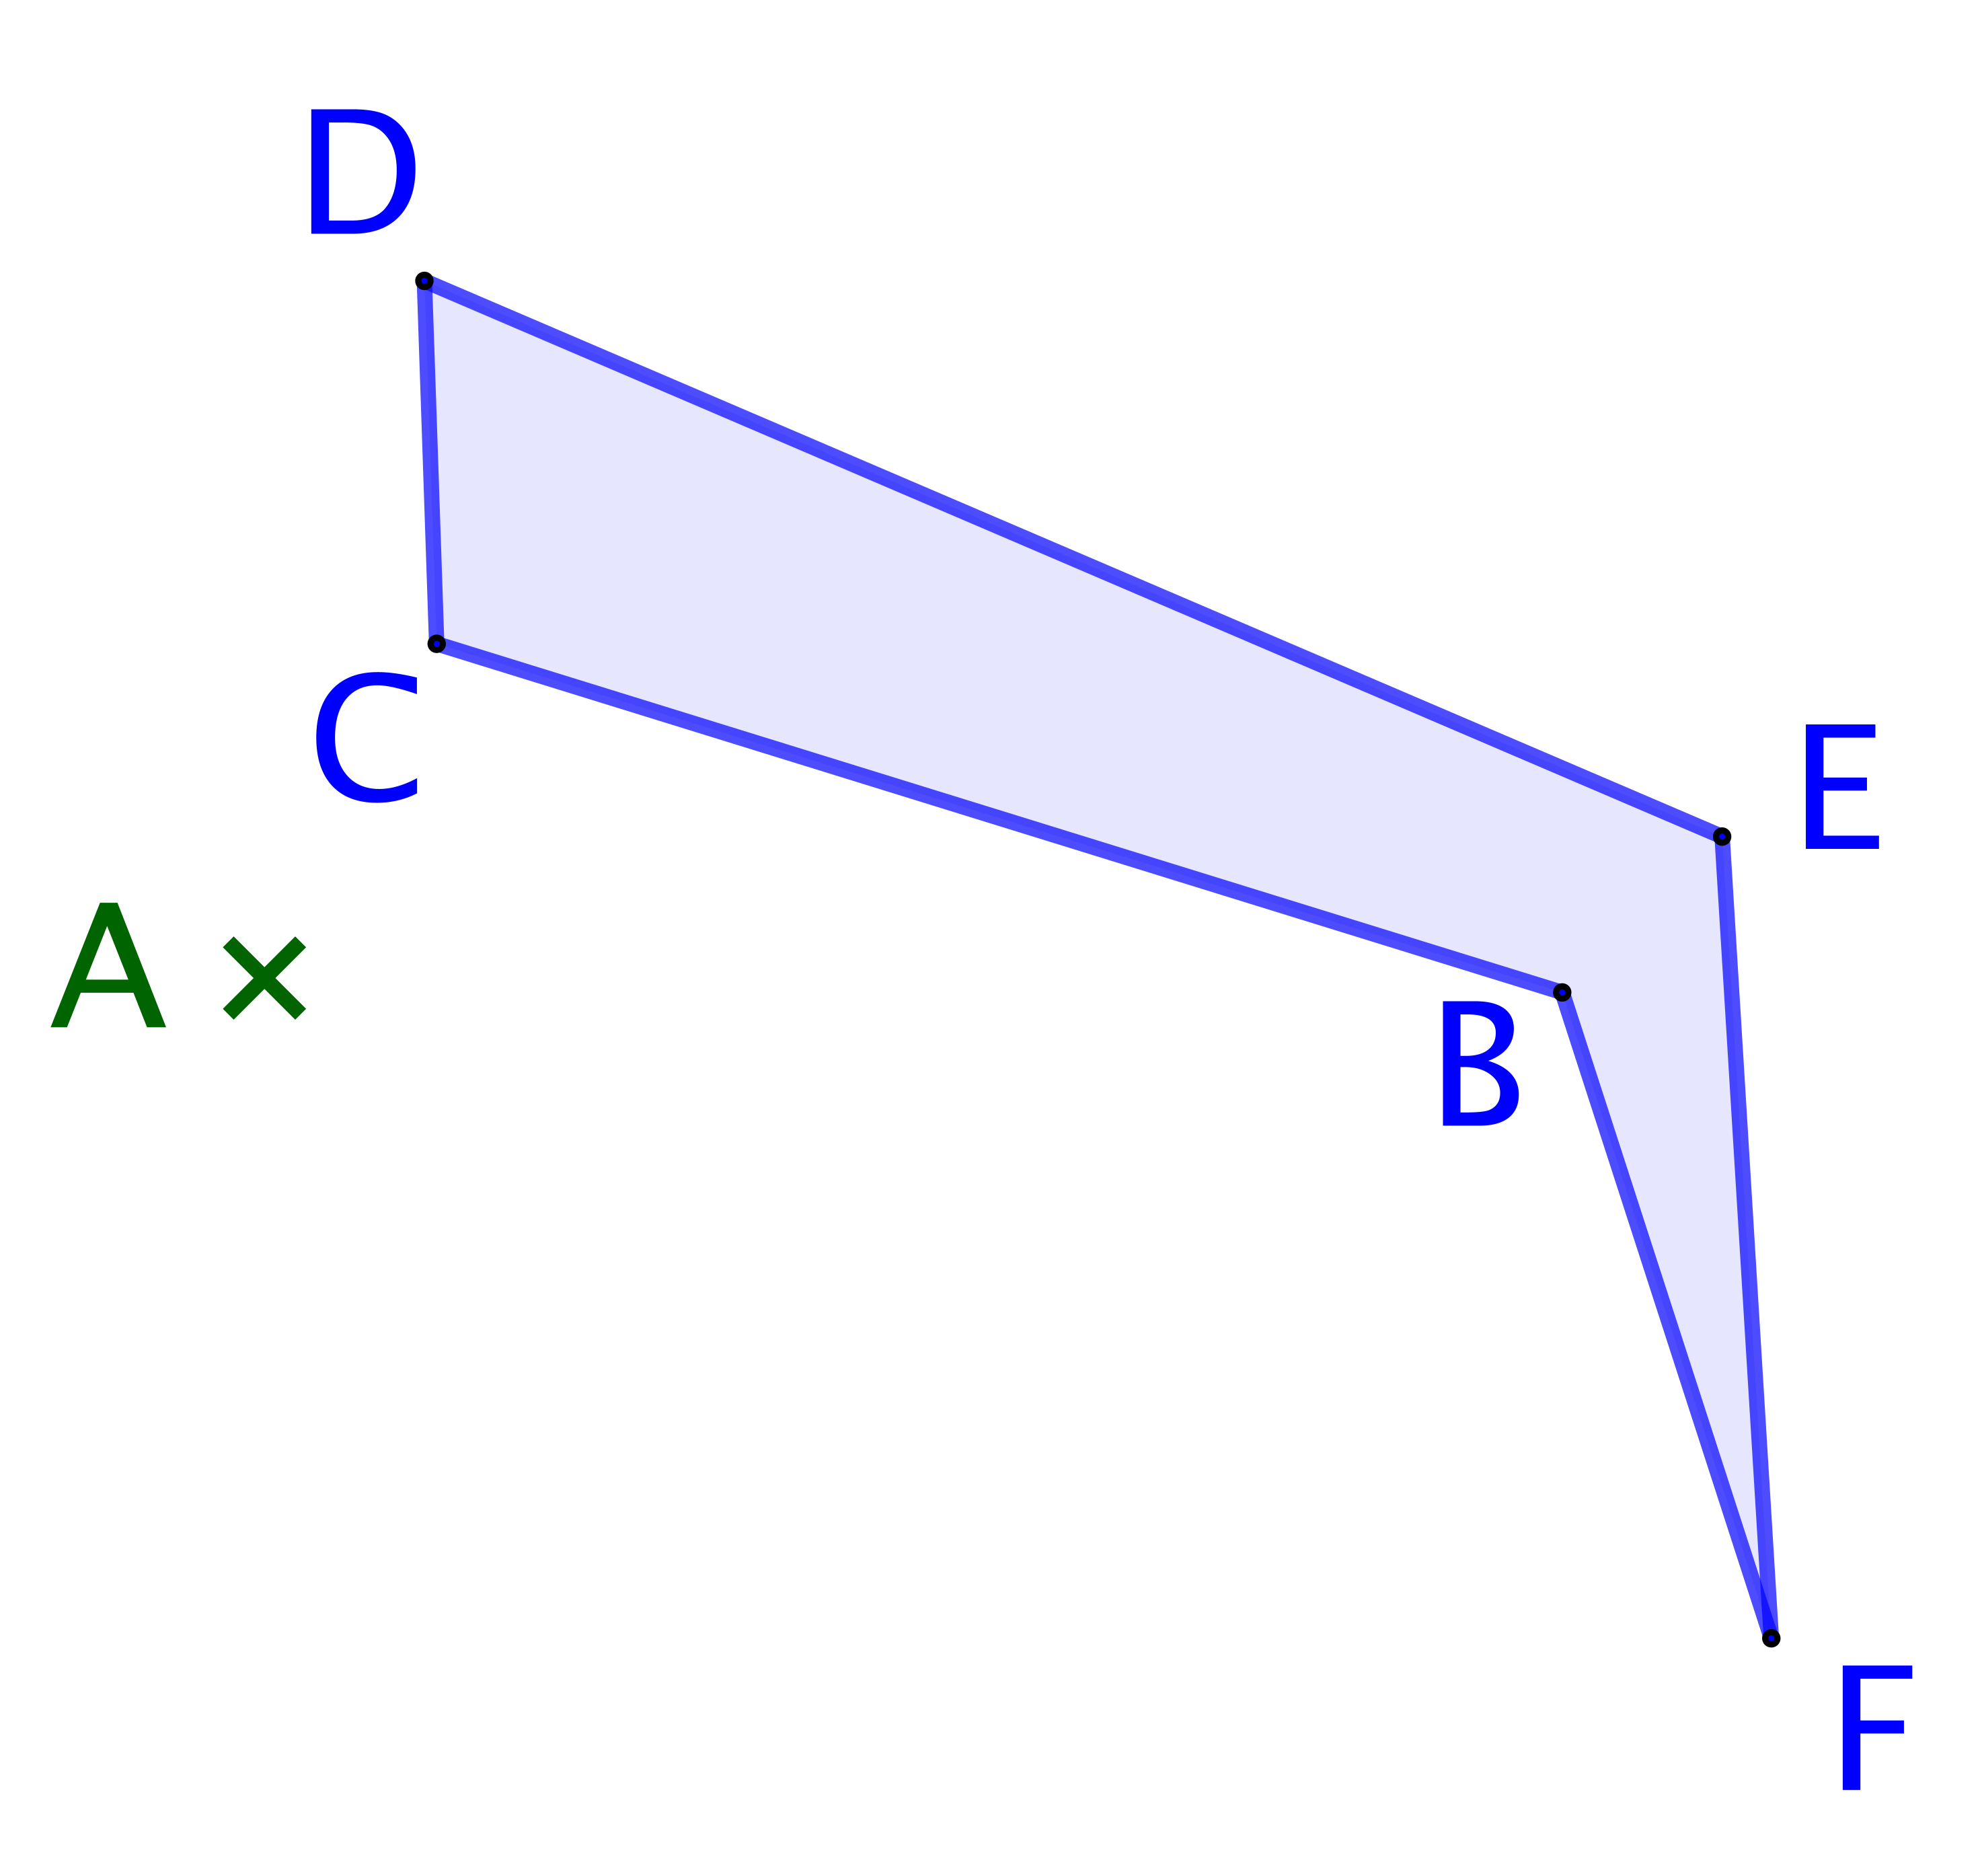
\includegraphics[scale=.4]{content/polygon/sufficient-cond/triangulation-3.png}
        
            \smallskip
            Le \ngone\ allégé.
        \end{center}
    \end{multicols}
    
    
    Le théorème de triangulation admet une forme forte donnant une décomposition contenant un triangle formé de deux côtés consécutifs du \ngone.%
    \footnote{
        En pratique, cette forme forte est peu utile, car elle aboutit à un algorithme de recherche trop lent.
    }
    Nous dirons qu'une telle décomposition est \og \emph{à l'écoute} \fg.
    Ce très mauvais jeu de mots fait référence à la notion sérieuse \og \emph{d'oreille} \fg\ pour un \ngone: une oreille est un triangle inclus dans le \ngone, et formé de deux côtés consécutifs du \ngone.
    L'exemple suivant donne un \ngone\ n'ayant que deux oreilles: ceci montre que l'existence d'une oreille ne va pas de soi.%
    \footnote{
        On démontre que tout \ngone\ admet au minimum deux oreilles.
    }


    \begin{multicols}{2}
        \small\itshape
    	\begin{center}
        	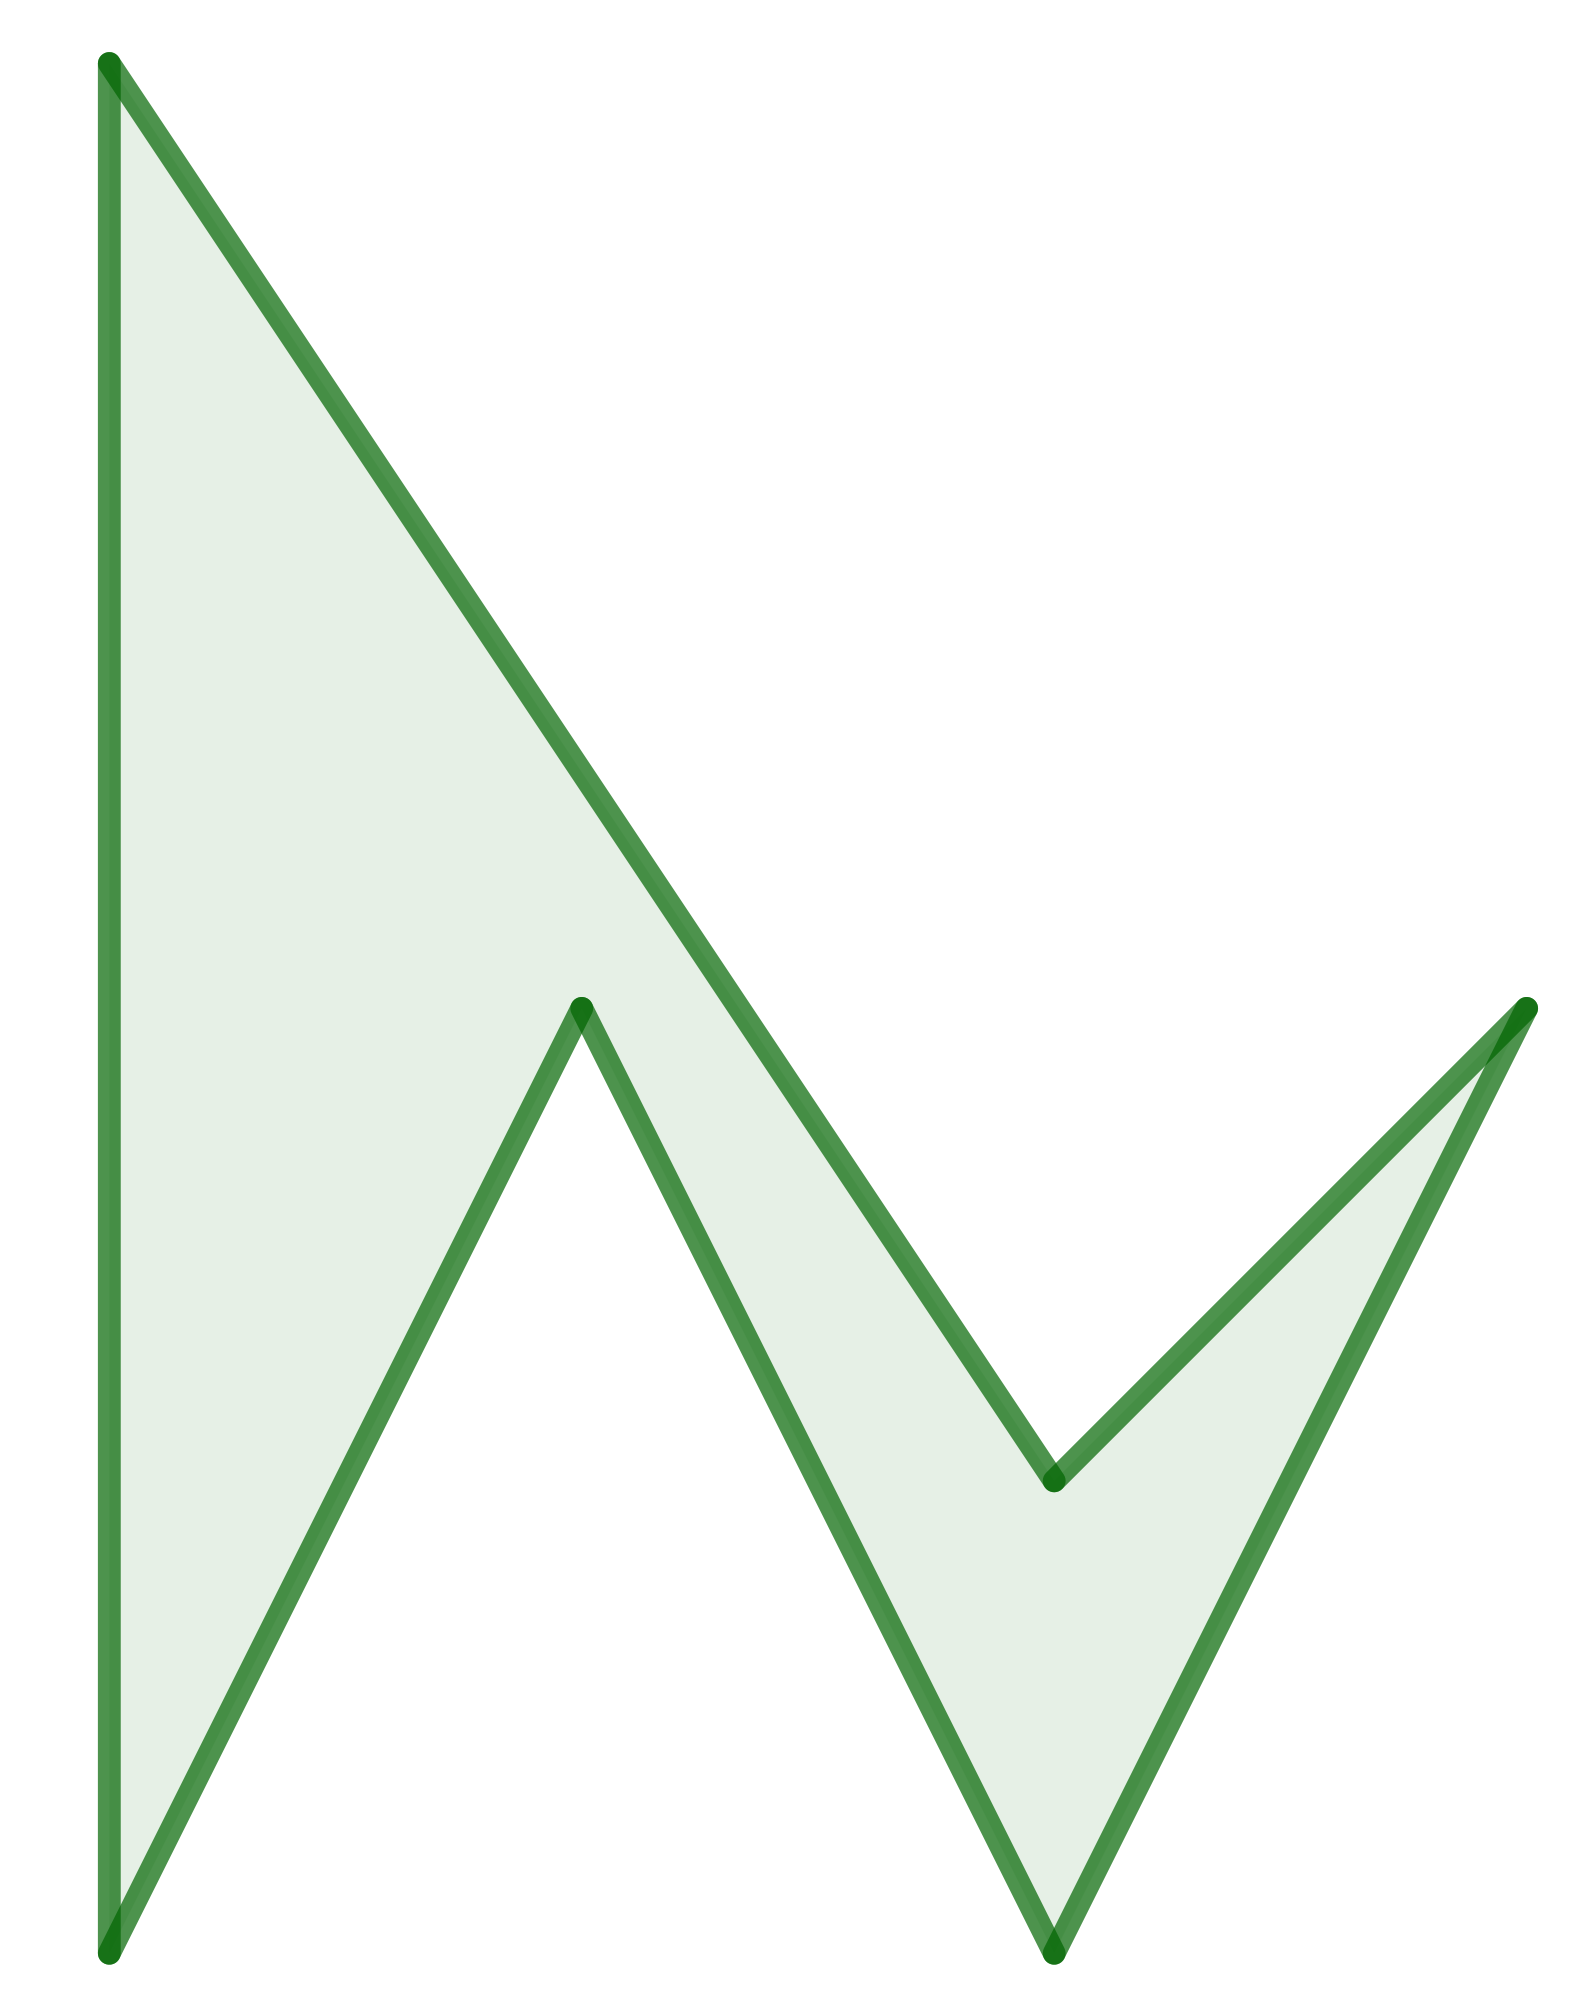
\includegraphics[scale=.4]{content/polygon/sufficient-cond/mini-ear-1.png}
        
        	\smallskip
       		Un \ngone\ basique.
    	\end{center}
	
    	\begin{center}
        	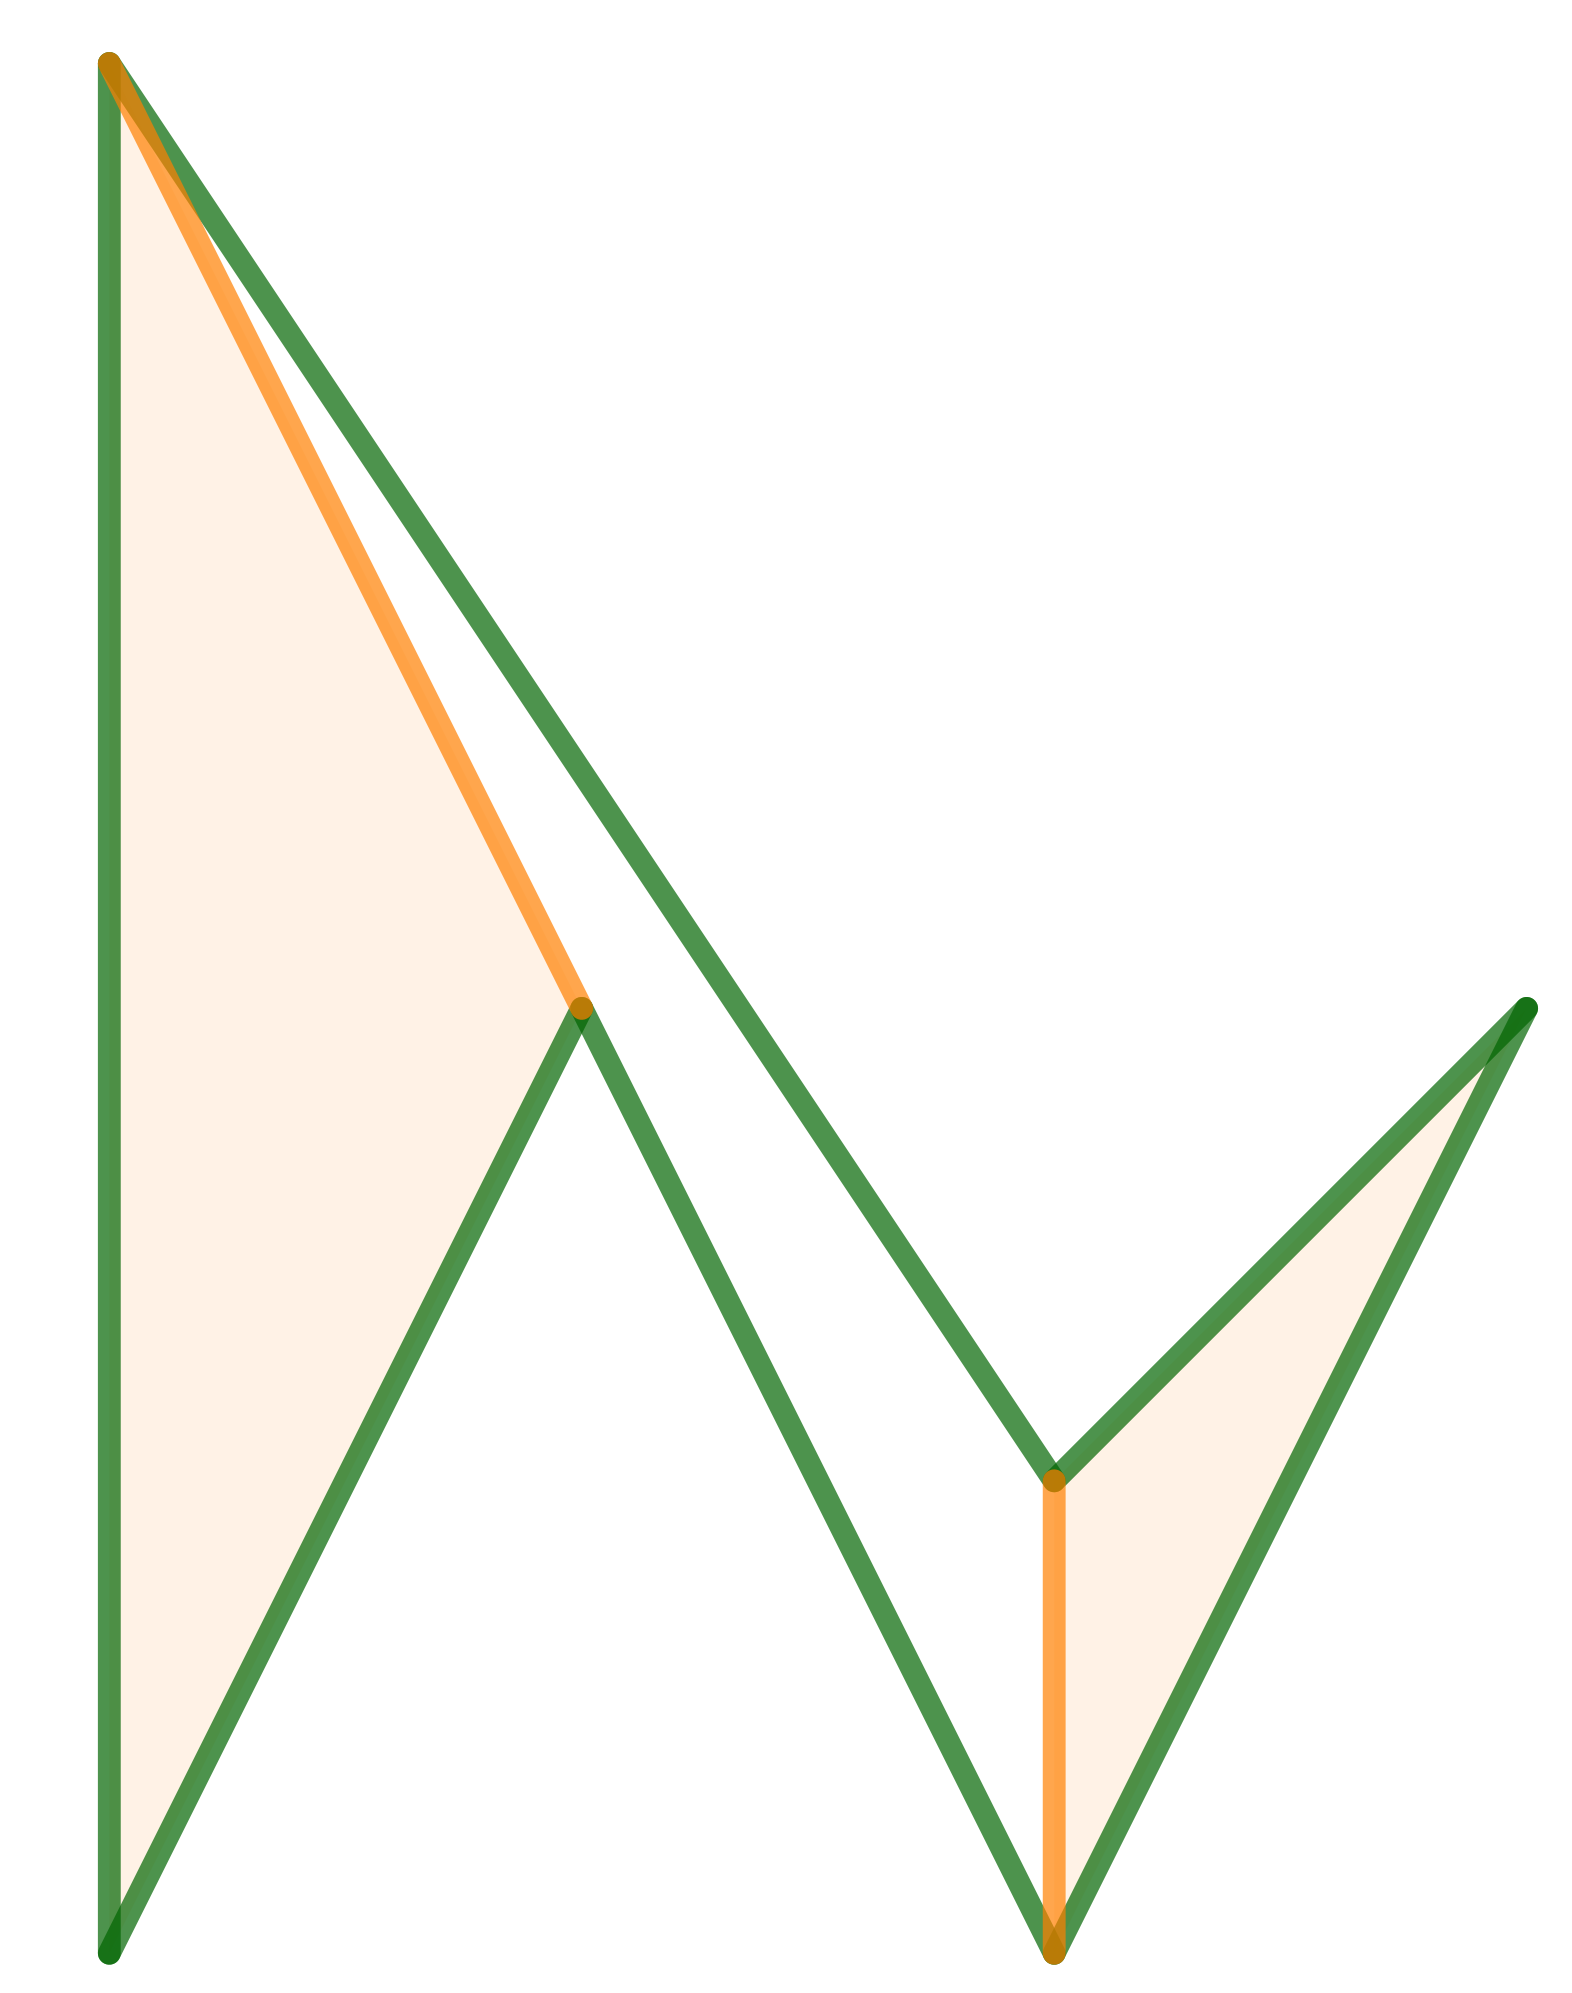
\includegraphics[scale=.4]{content/polygon/sufficient-cond/mini-ear-2.png}
        
        	\smallskip
       		Juste deux oreilles disponibles.
    	\end{center}
    \end{multicols}
    
    
    
    Soit $\setproba{P}$ un \ngone\ avec $n \geq 4$, et $\setproba{L} = A_1 A_2 \cdots A_n$ la \nline\ obtenue en parcourant la frontière de $\setproba{P}$ à partir d'un sommet $A_1$ tel que $A_1 A_{n-1} A_n$ soit une oreille de $\setproba{P}$.
    
    
    \begin{center}
        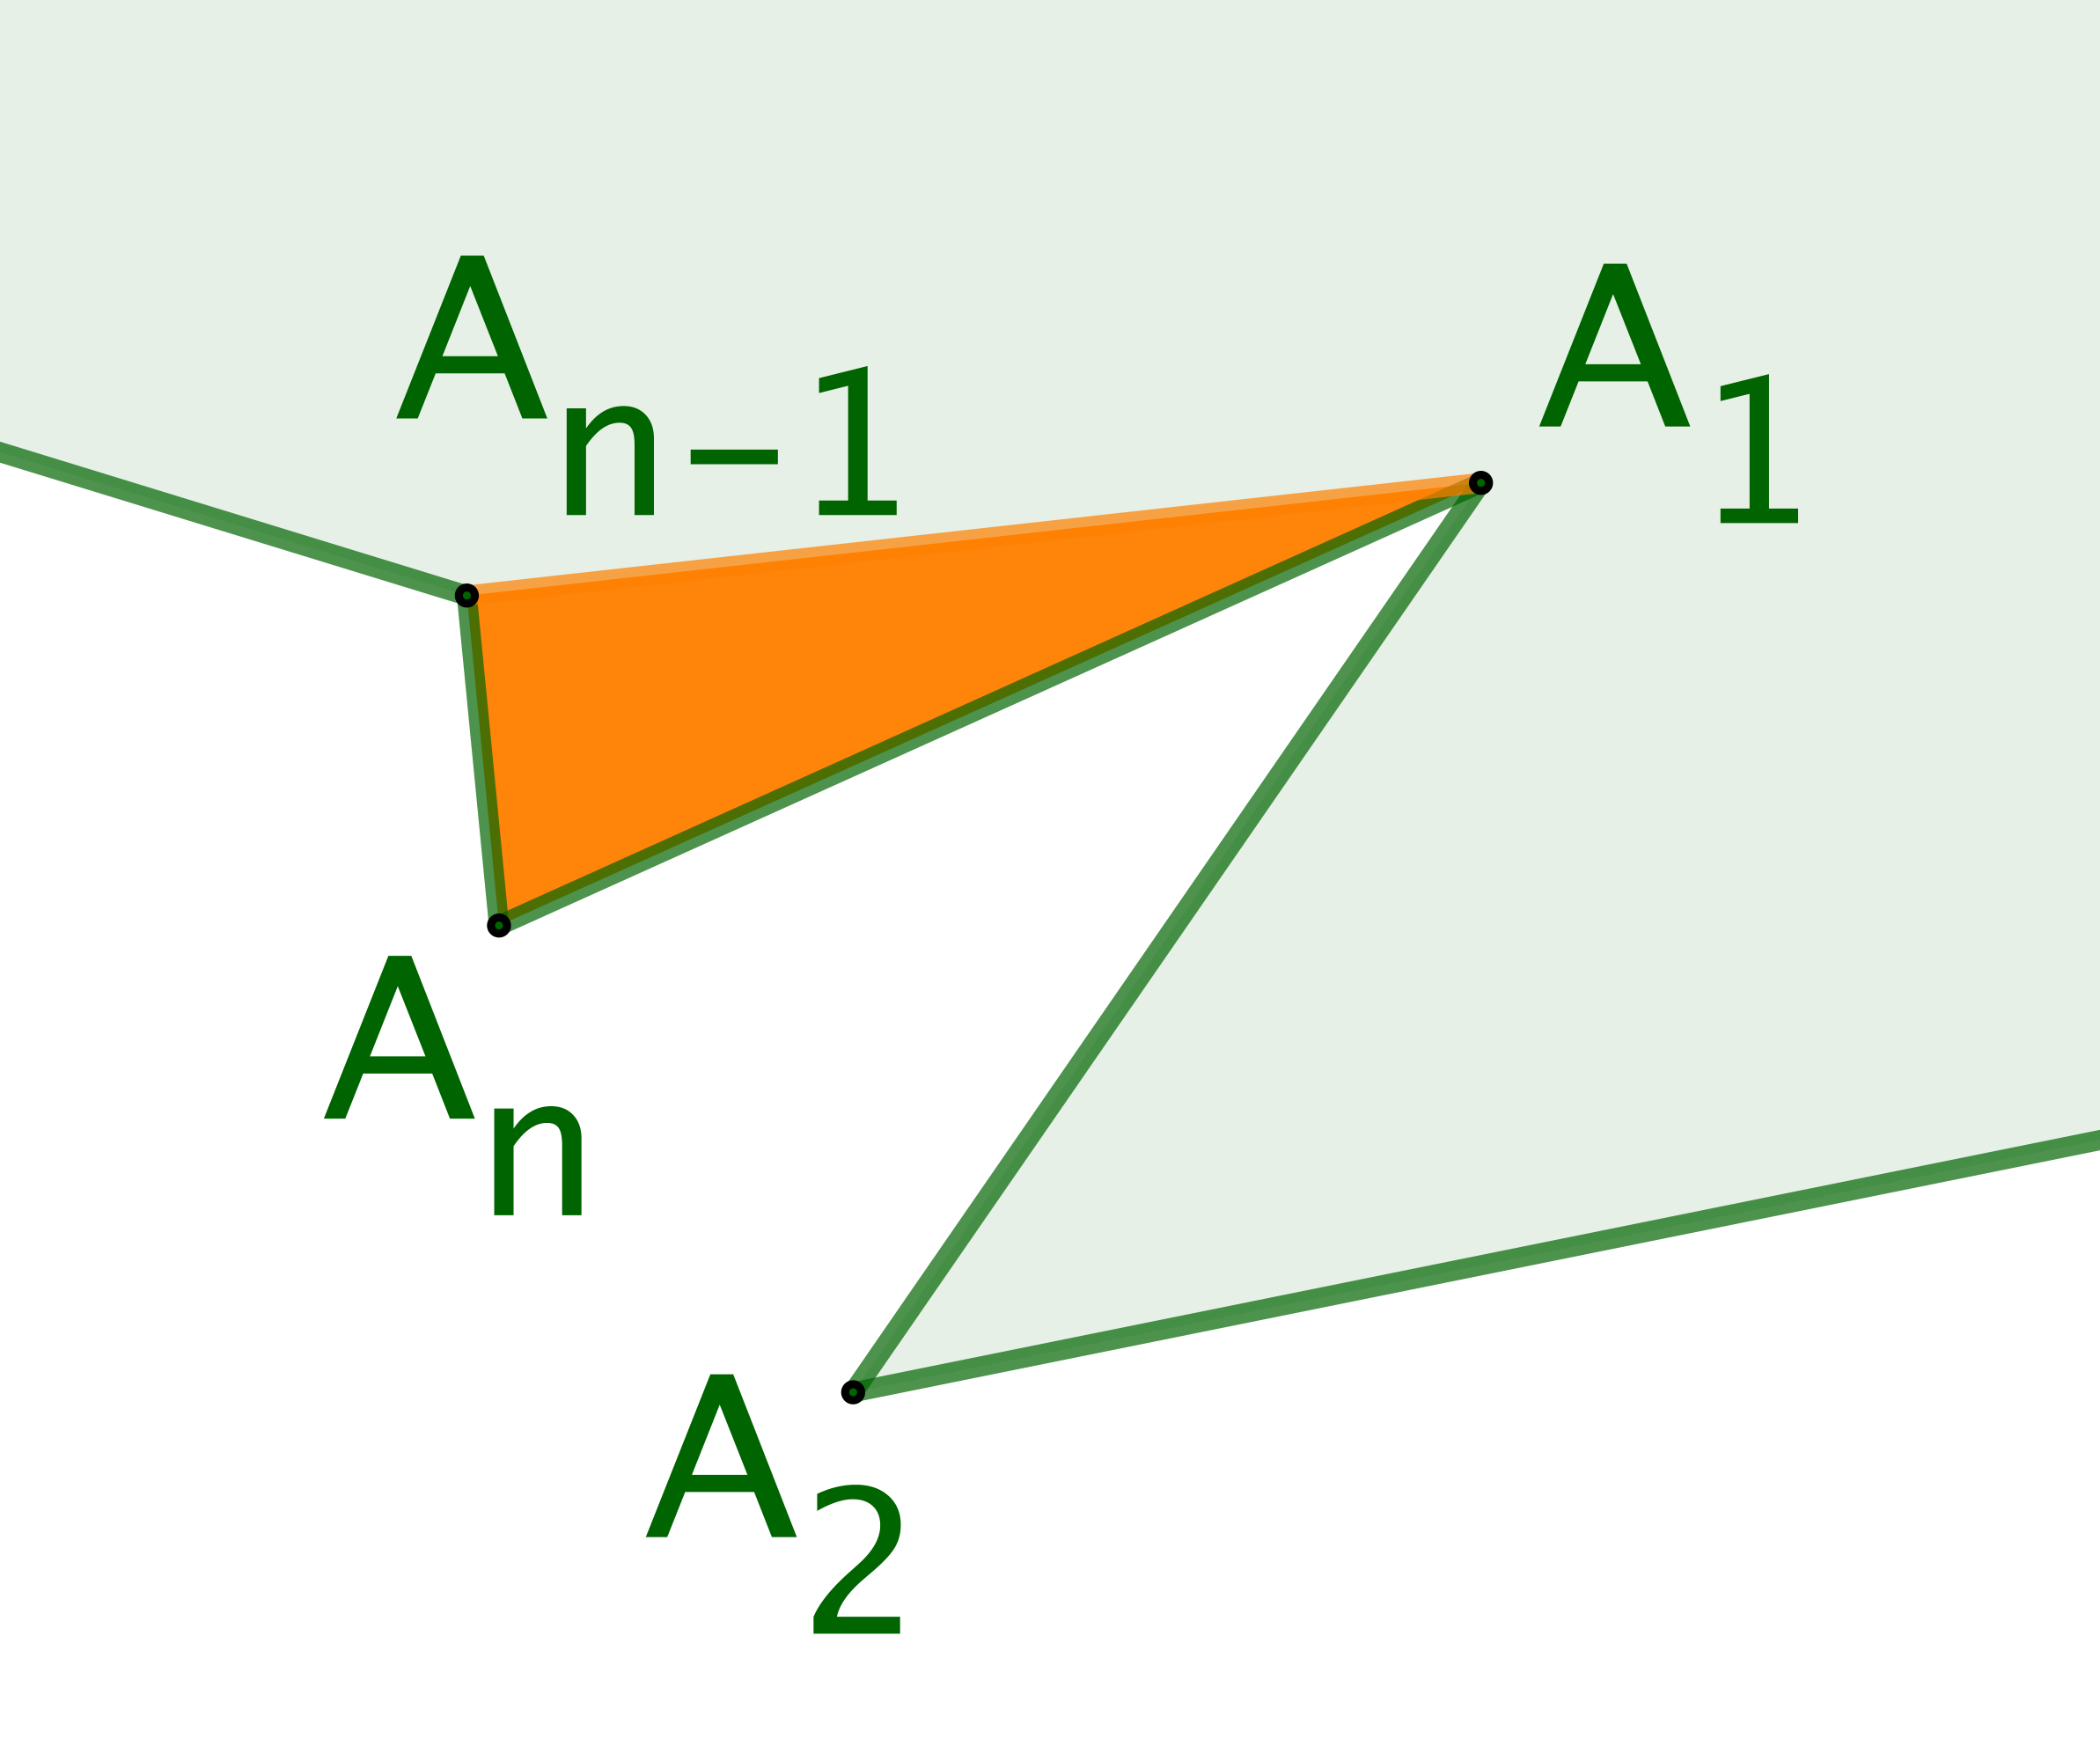
\includegraphics[scale=.4]{content/polygon/sufficient-cond/triangulation-proof.png}
    \end{center}
    
    
    Nous voilà prêt à raisonner par récurrence sur $n \in \NN_{\geq3}$.
    Le cas $n = 3$ ne posant aucune difficulté, nous allons juste considérer l'étape de récurrence en reprenant les notations précédentes.
    Soit ensuite
    $\setproba{P}^{\,\prime}$ le \kgone\ associé à la \kline\ $\setproba{L}^{\,\prime} = A_2 \cdots A_n$ où $k = n-1$ vérifie $k \in \NN_{\geq3}$.
    
    \begin{itemize}
    	\item $\area{\setproba{P}} = \area{A_1 A_{n-1} A_n}  +  \area{\setproba{P}^{\,\prime}}$, 
		car $A_1 A_{n-1} A_n$ est une oreille de $\setproba{P}$.


    	\item $\area{A_1 A_{n-1} A_n} = \garea{A_1 A_{n-1} A_n}$ et $\area{\setproba{P}^{\,\prime}} = \garea{\setproba{P}^{\,\prime}}$ 
		par récurrence.


    	\item Il n'est pas certain que $\garea{A_1 A_{n-1} A_n} + \garea{\setproba{P}^{\,\prime}} = \garea{\setproba{P}}$,
		du fait de l'utilisation de la valeur absolue pour définir une aire généralisée. Nous allons voir que c'est malgré tout le cas. 
		Quitte à changer de sens parcours de la frontière de $\setproba{P}$, et à renommer les sommets, 
		tout en utilisant $\Omega = A_n$ comme point de calcul,
		nous pouvons supposer que 
		$2 \garea{\setproba{P}^{\,\prime}}
		= \dsum_{j=1}^{n-2} \det \big( \vect{A_n A_j} , \vect{A_n A_{j + 1}} \big) 
		+ \det \big( \vect{A_n A_{n-1}} , \vect{A_n A_1} \big)$.
		Nous effectuons alors les calculs suivants.

		\leavevmode\kern-2em%
		\begin{stepcalc}[style=ar*]
			\pm 2 \garea{\setproba{P}}
		\explnext{Nous ne connaissons pas encore \\ le signe de la somme des déterminants.}
			\dsum_{j=1}^{n} \det \big( \vect{A_n A^{\,\prime}_j} ,  \vect{A_n A^{\,\prime}_{j + 1}} \big)
		\explnext{}
			\dsum_{j=1}^{n-2} \det \big( \vect{A_n A^{\,\prime}_j} , \vect{A_n A^{\,\prime}_{j + 1}} \big)
			+
			\det \big( \vect{A_n A^{\,\prime}_{n-1}} ,  \vect{A_n A^{\,\prime}_n} \big)
			+
			\det \big( \vect{A_n A^{\,\prime}_n} ,  \vect{A_n A^{\,\prime}_{n+1}} \big)
		\explnext*{$A_1 = A^{\,\prime}_{n+1}$ \\
		           $A_i = A^{\,\prime}_i$ \\ pour $i \leq n$}%
		          {}
			2 \garea{\setproba{P}^{\,\prime}}
			-
			\det \big( \vect{A_n A_{n-1}} , \vect{A_n A_1} \big)
		\explnext{}
			2 \garea{\setproba{P}^{\,\prime}}
			+
			\det \big( \vect{A_n A_1} , \vect{A_n A_{n-1}} \big)
		\end{stepcalc}
		
		\noindent
		Il faut donc justifier que nécessairement 
		$2 \garea{A_1 A_{n-1} A_n} = \det \big( \vect{A_n A_1} , \vect{A_n A_{n-1}} \big)$,
		car ceci donnera la positivité de la dernière somme qui sera donc égale à $2 \garea{\setproba{P}}$, puis nous aurons 
		$2 \garea{\setproba{P}} = 2 \garea{\setproba{P}^{\,\prime}} + 2 \garea{A_1 A_{n-1} A_n}$ 
		comme souhaité.
		
		
		
		XXXXX


    	\item Les points précédents donnent bien $\area{\setproba{P}} = \garea{\setproba{P}}$, ce qui achève notre démonstration par récurrence.
    \end{itemize}
\end{proof}


% ----------------------- %


\begin{fact} \label{no-cross-max}
    Si une \nline\ $\setproba{L}$ non dégénérée n'est pas un \ngone, donc est un polygone croisé, alors on peut construire un \ngone\ $\setproba{P}$ tel que 
	$\perim{\setproba{P}} = \perim{\setproba{L}}$ 
	et 
	$\garea{\setproba{P}} > \garea{\setproba{L}}$.
\end{fact}


\begin{proof}
	XXXX
\end{proof}



% ----------------------- %


\begin{fact} \label{suff-cond}
    Soit $n \in \NN_{\geq3}$ un naturel fixé.
    Considérons tous les \ngones\ de périmètre fixé. Parmi tous ces \ngones, il en existe au moins un d'aire maximale.
\end{fact}


\begin{proof}
	Ce qui suit nous donne plus généralement l'existence d'un \ngone, au moins, maximisant l'aire généralisée parmi toutes les \nlines\ de périmètre fixé $p$.
    %    
    \begin{itemize}
        \item On munit le plan d'un repère orthonormé direct $\pvaxes{O | i | j}$. 


        \item On considère $\setproba{Z}$ l'ensemble des \nlines\ $\setproba{L} = A_1 A_2 \cdots A_n$ vérifiant les propriétés suivantes.%
        \footnote{
        	Le mot \og \emph{Zeile} \fg\ est une traduction possible de \og \emph{ligne} \fg\ en allemand.
        }
        %
        \begin{enumerate}
        	\item $\perim{A_1 A_2 \cdots A_n} = p$

        	\item $A_1\coord{0 | 0}$
        \end{enumerate}


        \item Nous notons ensuite $\setproba{G} \subset \RR^{2n}$ l'ensemble des uplets $\big( x(A_1) ; y(A_1) ; \dots ; x(A_n) ; y(A_n) \big)$ correspondant aux coordonnées des sommets $A_i$ de \nlines\ appartenant à $\setproba{Z}$.
        
        
        \item $\setproba{G}$ est clairement fermé dans $\RR^{2n}$.
        De plus, il est borné, car les coordonnées des sommets des \nlines\ considérées le sont.        
        En résumé, $\setproba{G}$ est un compact de $\RR^{2n}$.


        \item Nous définissons la fonction $s: \setproba{G} \rightarrow \RRp$ qui à un uplet de $\setproba{G}$ associe l'aire généralisée de la \nline\ qu'il représente. 
        Cette fonction est continue comme valeur absolue d'une fonction polynomiale en les coordonnées.
       
        
        \item Finalement, par continuité et compacité, on sait que $s$ admet un maximum sur $\setproba{G}$.
        Or, un tel maximum ne peut être atteint en une \kline\ dégénérée, clairement, ni en un polygone croisé d'après le fait \ref{no-cross-max}, donc un tel maximum sera obtenu avec un \ngone. That's all folks!
    \end{itemize}    
\end{proof}


% ----------------------- %


\begin{fact}
    Soit $n \in \NN_{\geq3}$ un naturel fixé.
    Considérons tous les \ngones\  de périmètre fixé. Parmi tous ces \ngones, un seul est d'aire maximale, c'est le \ngone\ régulier.
\end{fact}


\begin{proof}
    Ceci découle directement des faits \ref{nece-cond} et \ref{suff-cond}.
    Ici s'achève notre joli voyage.
\end{proof}